%% ----------------------------------------------------------------
%% MAIN FILE (the one that you compile with LaTeX)
%% ---------------------------------------------------------------- 


% \documentclass[a4paper, 11pt, twoside, openright]{uis-thesis}
\documentclass[a4paper, 11pt]{uis-thesis}
\graphicspath{{figures/}}  % Location of the graphics files (set up for graphics to be in PDF format)

% Include any extra LaTeX packages required
\usepackage[square, numbers, comma, sort&compress]{natbib}  % Use the "Natbib" style for the references in the Bibliography
\usepackage{verbatim}  % Needed for the "comment" environment to make LaTeX comments
% \usepackage{vector}  % Allows "\bvec{}" and "\buvec{}" for "blackboard" style bold vectors in maths
\usepackage{algorithm}
\usepackage{algorithmic}
\usepackage[T1]{fontenc}
\usepackage{subfigure}
\usepackage{venturis2}
\usepackage{lmodern}
\usepackage{textcomp}    % solve issues with lmodern
\usepackage{amsfonts}
\usepackage{amsmath}
\usepackage{amsthm}
\usepackage{pdfpages}
\usepackage{microtype}   % better typesetting with pdfLaTeX
\usepackage[compact]{titlesec}
\usepackage{booktabs}
\usepackage{sectsty}     % section titles in specified font face
\usepackage{tikz}        % For drawing graphics
\usepackage{amsmath}

\DeclareMathOperator*{\argmax}{arg\,max}
\DeclareMathOperator*{\argmin}{arg\,min}

\allsectionsfont{\sffamily}
\numberwithin{algorithm}{chapter}
\setcounter{secnumdepth}{2}
\setcounter{tocdepth}{2}
\renewcommand{\captionlabelfont}{\sffamily\bfseries}
\newtheorem{thm}{Theorem}
\renewcommand{\algorithmicrequire}{\textbf{Input:}}
\renewcommand{\algorithmicensure}{\textbf{Output:}}
\hypersetup{urlcolor=blue, colorlinks=true}  % Colours hyperlinks in blue, but this can be distracting if there are many links.

\newcommand{\todo}[1]{\textcolor{red}{#1}}
\newcommand{\instructions}[1]{\textcolor{blue}{#1}}


\listfiles

%\usepackage[draft]{hyperref}
%\usepackage[hyperfootnotes=false,plainpages=false]{hyperref}
%% ----------------------------------------------------------------
\begin{document}
\frontmatter	  % Begin Roman style (i, ii, iii, iv...) page numbering
% Fill your name and supervisor name and sign it and replace the frontpage.
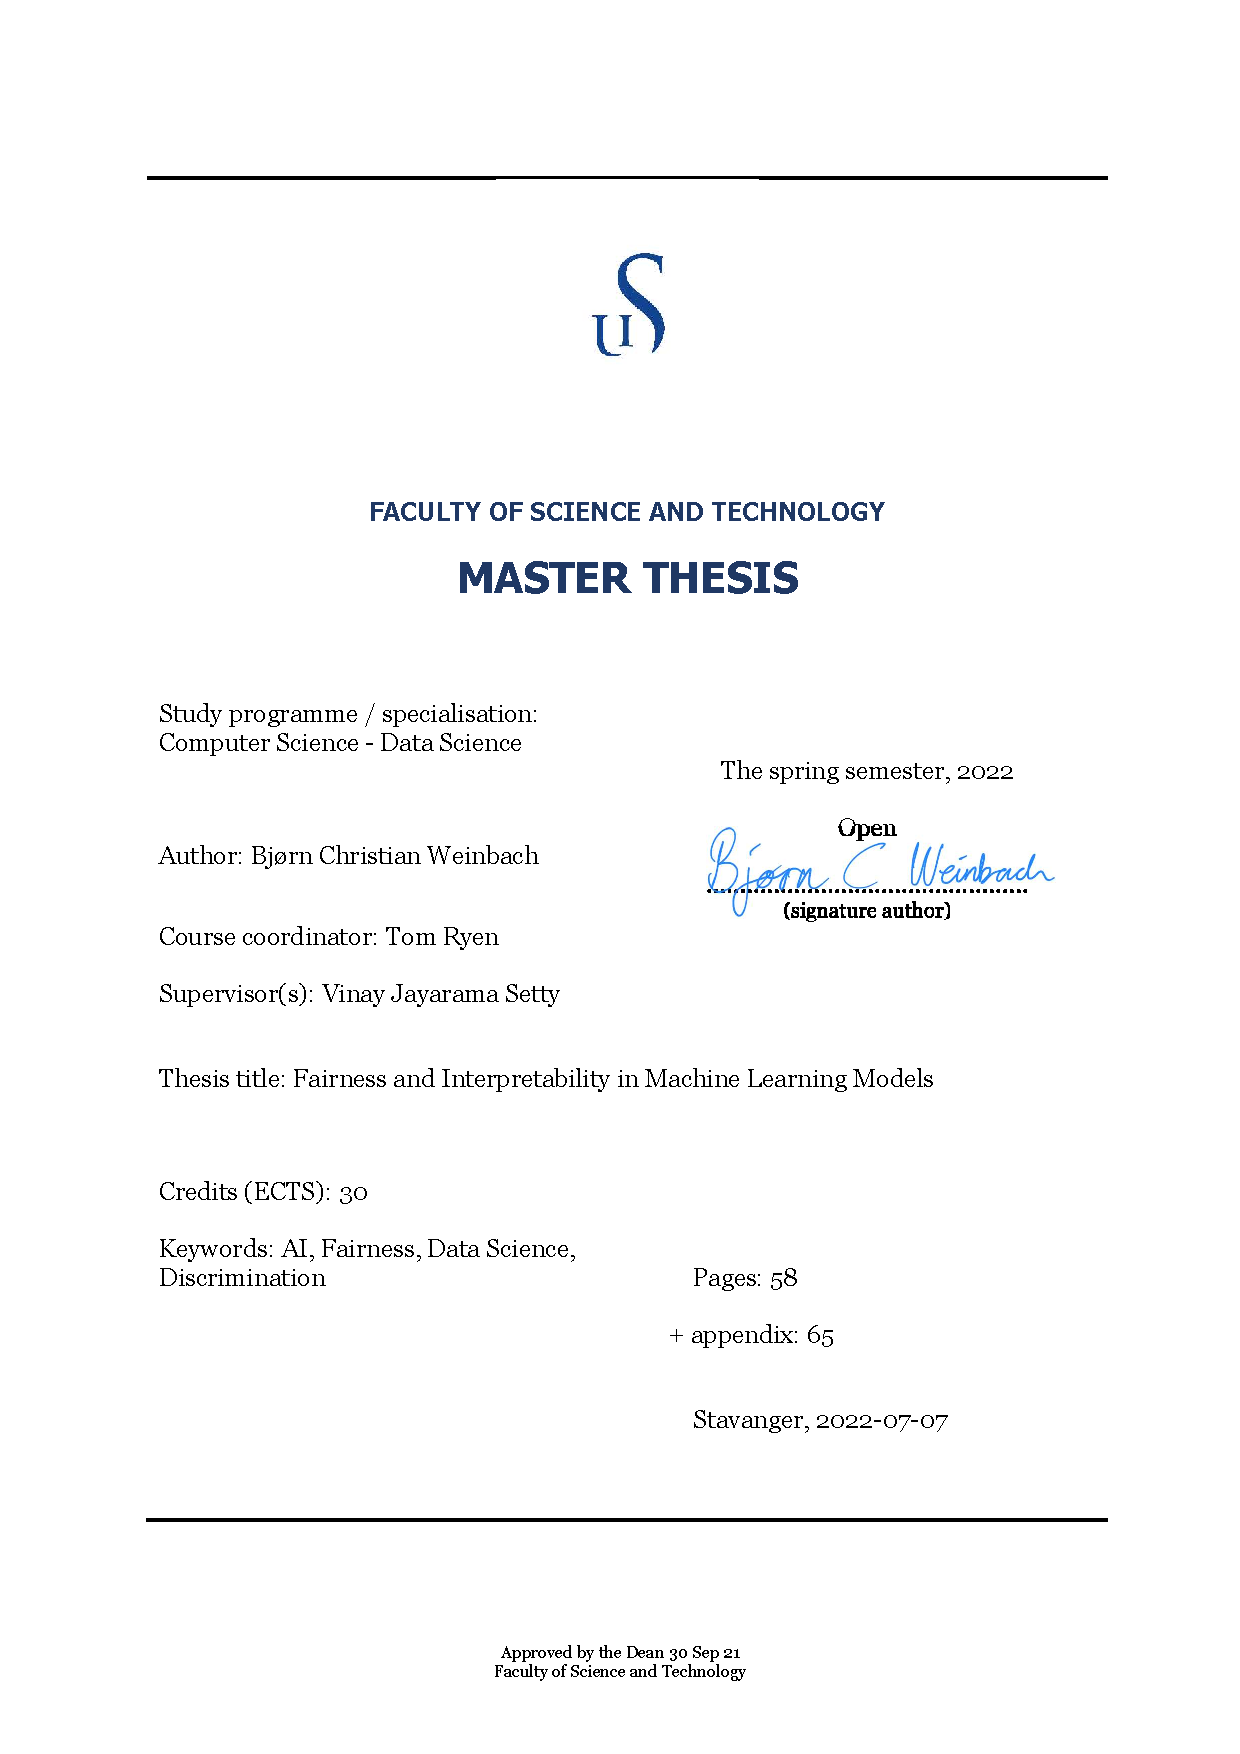
\includepdf[offset=25mm -25mm, scale=1]{./frontpage-masters.pdf}


\title{Thesis Title}
\authors{Weinbach Bjørn Christian}
\addresses{\groupname\\\deptname\\\univname}  % Do not change this here, instead these must be set in the "Thesis.cls" file, please look through it instead
\date       {\today}
\subject    {}
\keywords   {}

\maketitle
%% ----------------------------------------------------------------

\setstretch{1.3}  % It is better to have smaller font and larger line spacing than the other way round

% Define the page headers using the FancyHdr package and set up for one-sided printing
%\fancyhead{}  % Clears all page headers and footers
%\rhead{\thepage}  % Sets the right side header to show the page number
%\lhead{}  % Clears the left side page header

% \pagestyle{fancy}  % Finally, use the "fancy" page style to implement the FancyHdr headers
% \fancyhead[RE,LO]{\sffamily\bfseries\nouppercase{\rightmark}}
% \fancyhead[LE,RO]{\thepage}


%% ----------------------------------------------------------------
\pagestyle{empty}  % No headers or footers for the following pages
% % % Declaration Page required for the Thesis, your institution may give you a different text to place here
% \Declaration{

% \addtocontents{toc}{\vspace{1em}}  % Add a gap in the Contents, for aesthetics

%TODO: use macro for authors; if multiple, we should say "We" instead of "I"
% I, Vinay Setty, declare that this thesis titled, `Efficiently Identifying Interesting Time Points in Text Archives' and the work presented in it are my own. I confirm that:

% \begin{itemize} 
% \item[\tiny{$\blacksquare$}] This work was done wholly or mainly while in candidature for a master's degree at this University.
  
% \item[\tiny{$\blacksquare$}] Where I have consulted the published work of others, this is always clearly attributed.
 
% \item[\tiny{$\blacksquare$}] Where I have quoted from the work of others, the source is always given. With the exception of such quotations, this thesis is entirely my own work.
 
% \item[\tiny{$\blacksquare$}] I have acknowledged all main sources of help.

% \end{itemize}
%  \vspace{5pt}
% Signed:\\
% \rule[1em]{25em}{0.5pt}  % This prints a line for the signature
 
% Date:\\
% \rule[1em]{25em}{0.5pt}  % This prints a line to write the date
% }
% \clearpage  % Declaration ended, now start a new page

% \clearpage
\null\vfill
% Now comes the "Funny Quote", written in italics
\textit{``Programming is a nice break from thinking.''}

\begin{flushright}
Leslie Lamport
\end{flushright}

\vfill\vfill\vfill\vfill\vfill\vfill\null

\clearpage
\addtotoc{Abstract}  % Add the "Abstract" page entry to the Contents
\abstract{
\addtocontents{toc}{\vspace{1em}}  % Add a gap in the Contents, for aesthetics

}

\clearpage

\setstretch{1.3}  % Reset the line-spacing to 1.3 for body text (if it has changed)

% The Acknowledgements page, for thanking everyone
\acknowledgements{
\addtocontents{toc}{\vspace{1em}}  % Add a gap in the Contents, for aesthetics
I would like to thank my supervisors for their fantastic enthusiasm and help with writing this thesis. 

}

\clearpage

\tableofcontents

\setstretch{1.3}  % Return the line spacing back to 1.3

\addtocontents{toc}{\vspace{2em}}  % Add a gap in the Contents, for aesthetics

%% ----------------------------------------------------------------
\mainmatter	  % Begin normal, numeric (1,2,3...) page numbering
\pagestyle{fancy}  % Return the page headers back to the "fancy" style

% Include the chapters of the thesis, as separate files
% Just uncomment the lines as you write the chapters


\chapter{Introduction}
\label{ch:intro}

\section{Background and Motivation}

\label{sec:intro:background}

Presently, we are undergoing both the Information Age and the fourth industrial revolution \citep{Castells:2009:Book, Hamdan:2021:Book}. The information age has been characterised by the commercialisation of computer power resulting from technological advances in transistor technology and global communication technologies \citep[p.~30]{Castells:2009:Book}. The fourth industrial revolution is marked by growing connectivity and intelligent automation \citep{Bai:2020:IJPE}. Modern smart technology, large-scale machine-to-machine communication (M2M), and the internet of things (IoT) are causing fundamental shifts in the global production and supply network as old manufacturing and industrial methods continue to be automated. 

In this broader technological advancement, machine learning has become only one of several fields. In particular, machine learning is replacing manual labour through automation and robotics, as well as higher-level decision-making by quantifying large-scale data and applying this information to provide insight to human decision-makers \citep{Hamdan:2021:Book}.

The way we do business is changing rapidly. Machine learning is becoming more embedded into our lives, working behind the scenes in diverse scenarios, from optimising production yield to recommending products and more. This shift has enhanced awareness about the implications of using machine learning in numerous processes, as well create more demand to make machine learning powered decisions more fair and interpretable.

These transformations are required to meet many of the UN-defined sustainability goals, such as affordable and clean energy, decent work and economic growth, and industry, innovation, and infrastructure (goals 7, 8, and 9, respectively) \citep{Bai:2020:IJPE}. In addition to these goals, the United Nations has outlined two others: gender equality and reduced disparities, goals 5 and 10, respectively \citep{UN:2015:Resolution}. In machine learning research, equality and fairness are consequently receiving a great deal more focus than in the past \cite{Mehrabi:2021:CSUR}.

Discrimination is when people are treated unfairly because of the groups, classes, or other categories to which they belong or are seen to belong. In terms of machine learning, there are many distinct definitions of discrimination \citep{Altman:2011:doc} and the fairness that one wants to attain to avoid this prejudice \citep{Binns:2018:PMLR}.

According to \citet{Dressel:2018:AAAS}, a real world example of discrimination in terms of machine learning is COMPAS (Correctional Offender Management Profiling for Alternative Sanctions). A frequently used technique for determining criminal risk. Since its inception in 1998, it has been used to examine over 1 million offenders. COMPAS uses 137 factors about a person and their criminal history to forecast whether they would commit a misdemeanour or felony within two years of being assessed.

One would think that ignoring sensitive groups, classes, or other categories would be an easy method to avoid discrimination. Counterintuitively, omitting sensitive attributes is insufficient to eliminate prejudice. The discriminatory decision rule is learned indirectly by the machine learning model from qualities that correlate to the sensitive one \citep{Dressel:2018:AAAS, Calders:20210:DMKD}. This process is called redlining. The sensitive attribute must be included to penalise the machine learning model when it discriminates.

The source of bias and discrimination often comes from the data that the machine learning algorithm is trained on. According to \citet{Mehrabi:2021:CSUR} some prominent sources of bias are

\begin{itemize}
    \item \textbf{Historical Bias}: Historical bias is the already existing bias and sociotechnical issues in the world. This affect the data generation process. Imagine trying to make a decision-making system for accepting people to a certain education institution. This system looks at data on previous admissions. From this data, it seems that men dominates studies like engineering. While this data is correct and reflects the current reality, the question remains on whether the system should reflect this reality in its decision-making.

    \item \textbf{Representation Bias}: Lack of representation of certain groups in datasets skew the dataset from the real-world distribution. This bias arises when the sample does not reflect the subgroups in the population that we make inference on. A well known example of this is in image classification, where men, white people and people from the western world have dominated image datasets. This means that other ethnicities, especially black women, suffer from discrimination from systems using image data for training \cite{Walsh:2022:ACM}.

    \item \textbf{Simpsons Paradox}: Bias originating from the analysis of heterogeneous data that is composed of subgroups or individuals with different behaviours. The best known example of this bias is from the University of California, Berkeley. Examination of aggregate data on graduate admissions to the University of California, Berkeley, for fall 1973 shows a clear but misleading pattern of bias against female applicants. The problem was that the analysis did not take into account that women tended to apply for departments that were very competitive and men applied for departments that were less competitive. When disaggregating the data this relationship disappears and a small favour towards women was shown \cite{Bickel:1975:Science}.
\end{itemize}

Data, especially big data, is often heterogeneous, generated by subgroups with their own characteristics and behaviours. The heterogeneity can bias the data. A model learned on biased data may lead to unfair and inaccurate predictions.

There are currently several challenges in the field of fair machine learning to face. Since ignoring the sensitive attributes does not help to mitigate bias, one must discover how to best employ these sensitive attributes to achieve fairness. In the literature, there exists several statistical and mathematical definitions of fairness. Rather concerning is the fact that some of these definitions are mathematically impossible to satisfy simultaneously \citep{Kleinberg:2017:LIPIcs}.

As of the time of writing this thesis, there is no gold standard on how to train fairness-aware machine learning algorithms, and there exists several approaches on how to achieve this \citep{Mehrabi:2021:CSUR}. The goal of this thesis is to explore some of these approaches and see how they compared to others. 

\section{Objectives}
\label{sec:intro:objectives}

The goal of this thesis is to explore certain models and approaches to achieve fairness-aware machine learning systems. Specifically, the thesis has the following objectives

\begin{itemize}
    \item Discover how probabilistic machine learning and graphical models can be used to model the discrimination process.
    \item Discover how probabilistic machine learning and graphical models can be used to quantify uncertainty in the model and its fairness.
    \item Explore what definitions of fairness are most appropriate for probabilistic machine learning.
    \item How does the probabilistic approach compare to traditional machine learning methods?
    \item Are the fair machine learning models explainable?
\end{itemize}

\subsection{RQ1: What probabilistic graphical model is most appropriate to model the discrimination process?}

Probabilistic machine learning models come in many different forms. In this thesis we want to use probabilistic machine learning to model the discrimination and data generation process. This is explained in further detail in Section~\ref{ch:related}. At the end, a specific probabilistic graphical model should be provided.

\subsection{RQ2: Are the proposed models explainable?}

Training a machine learning model to be able to learn decision rules that minimise some mathematical definition of fairness is one thing, but how does the model use the sensitive attributes in its decisions? The proposed fairness-aware models should be evaluated in terms of fairness and explainability as well. 

\subsection{RQ3: Are probabilistic machine learning models cost-effective?}

The probabilistic model proposed in this thesis should be compared to baseline methods to see if there are any benefits in terms of performance, accuracy, fairness as well as adding the Bayesian perspective to the problem. There should be a statistically significant increase in accuracy and fairness to justify the additional complexity in computation to be considered cost-effective. At the end, simulations should be presented with both real world datasets and synthetic datasets and their respective performance metrics.

\section{Approach and Contributions}
\label{sec:intro:approach}

In this thesis, different algorithms and methods have been explored. These have all been made into a python package for ease of use. This python package has been named Forseti, named after the Norse god of justice and reconciliation. This python package has several modules with implemented algorithms. The code and relevant documentation is available in the following github repository \footnote{\url{https://github.com/bcwein/Forseti}}, as well as attached to this thesis when submitted.

Later, the machine learning models are investigated whether they are interpretable. Feature Importance is calculated and Individual Conditional Expectation Plots are performed on the models to explain how the models are using the sensitive attributes in their decision making. This way we hope to gain better insight into how the fair models change their decision compared to their traditional counterparts.

We find that while models satisfy some definition of fairness, when one looks into the models decision making, one quickly realise if this increase in fairness scores is due to reducing model accuracy and predicting randomly or if the model actively uses the data in its decision making and is trying to learn fairer predictions. 

\section{Outline}
\label{sec:intro:outline}

In this section we have discussed the broader picture of machine learning and the current technological and economic developments in the world. Especially how fairness is becoming evermore important in society as a whole. Through this we have defined some research questions (RQs) that we want to explore.

In chapter~\ref{ch:related} we go into more detail on the related works and previous methods already developed. We go into detail on how they work and what described the mechanisms behind them. Chapter 2 serves to give you the necessary background knowledge to understand the workings in later chapters.

Chapter~\ref{ch:approach} describes the approach that is used in this thesis. We describe the software developed and how it is organised, how the experiments have been set up and how you can set this up on your own system. This chapter gives you the necessary insight to follow the approach yourself and understand exactly how the work in this thesis has been done.

Next in chapter~\ref{ch:eval} we show the results from the approach described in chapter~\ref{ch:approach}. This includes data exploration, experimental results, presentation of hypothesis tests and discussion of these results. 

Finally in chapter~\ref{ch:conclusion} we draw the final remarks. Including what we have found out, what has been good about the approach and our results and what are the limitations of this study. And finally, we conclude and propose possible future work.
\chapter{Related Work}
\label{ch:related}

One of the most important papers out there for getting to know the field of fairness in machine learning is the survey paper by \citet{Mehrabi:2021:CSUR}. This paper serves as a gateway to a lot of the current research in the field, a lot of which will be summarised in this section of the thesis.

\section{Bias in Data}

In Section~\ref{ch:intro} we discussed some sources of bias. Here we will go through more of them and in more detail. We have the following biases according to \citet{Mehrabi:2021:CSUR}:

\subsection{Historical Bias}

Historical Bias is the already existing bias and sociotechnical issues in the real word. These issues affect the data-generation process. So even given a perfect sampling method, the bias in the dataset will still exist. \cite{Suresh:2019:arXiv}

\subsection{Representation Bias}

This bias occurs as a by-product of the way we sample from the population. \cite{Suresh:2019:arXiv} Data collection is a non-trivial task and sampling a diverse dataset across large geographical regions and taking into account diversity in terms of race, culture, gender etc will in many cases not be possible. Still, the dataset will suffer from not representing the true distributions in the population.

\subsection{Measurement Bias}

This source of bias originates in the way the particular features were measured and utilised. \cite{Suresh:2019:arXiv} An example of this would be to use salary as a feature to assess risk of defaulting on a loan. This feature will be biased towards women since women has historically experienced having lower salaries than men.

\subsection{Population Bias}

Population bias arises when the sampled population have different properties than the original target population. \cite{Olteanu:2019:FDATA} An example of this would be to sample data from different social media platforms, which have different user demographics. I.e., men using Reddit and women using Instagram.

And there are many other sources of bias, and some of these are very hard to avoid. It is reasonable to assume that most available datasets today are biased, which makes the approach described in Section~\ref{sec:probmac} important.

\section{Algorithmic Fairness}

Many definitions of discrimination exist, and while there is no gold-standard, it is often defined as an absence of any prejudice or favouritism towards individuals or groups based on some intrinsic traits. \cite{Mehrabi:2021:CSUR, Nripsuta:2019:AIES} These definitions are core in the many mathematical definitions of fairness. Some of these are summarised below

\textbf{Equalized Odds}: According to \citet{Mehrabi:2021:CSUR, Hardt:2016:NIPS} A predictor $\hat{Y}$ satisfies equalised odds with respect to a sensitive attribute $A$ and outcome $Y$ if $\hat{Y}$ and $A$ are conditionally independent on $Y$. i.e.

\begin{equation*}
    P(\hat{Y}|A=0, Y=y) = P(\hat{Y}|A=1, Y=y), y \in {0, 1}
\end{equation*}

\textbf{Equal Opportunity}: According to \citet{Mehrabi:2021:CSUR, Hardt:2016:NIPS} A binary predictor $\hat{Y}$ satisfies equal opportunity with respect to $A$ and $Y$ if

\begin{equation*}
    P(\hat{Y}=1|A=0, Y=1) = P(\hat{Y}=1|A=1, Y=1)
\end{equation*}

\textbf{Demographic Parity}: According to \citet{Mehrabi:2021:CSUR, Dwork:2012:ITCS} A predictor $\hat{Y}$ satisfies demographic parity if 

\begin{equation}
    P(\hat{Y}|A=0) = P(\hat{Y}|A=1)
    \label{eq:dempar}
\end{equation}

And many more metrics exist. A challenge is that according to \citet{Mehrabi:2021:CSUR, Kleinberg:2017:LIPIcs} it is impossible to satisfy some of these fairness constraints. One should therefore be considerate when using a certain metric. Synthesising these definitions to one gold-standard remains an open research question. For this thesis. Demographic parity is especially important as it is fundamental to the model described in Section~\ref{sec:paper1}.

\textbf{Strong Demographic Parity}: According to \citet{Antonio:2021:arXiv}, this is a parity score that extends demographic parity by considering fairness throughout the entire range of possible decision thresholds. It was proposed by \citet{Jiang:2020:PMLR}. When learning a fair classifier to satisfy strong demographic parity, the predictor $\hat{Y}$ must satisfy demographic parity for any threshold $t$ and sensitive attribute $A$

$$
\forall t \in \hat{Y} : P(\hat{Y} \geq t | A = 0) = P(\hat \geq t | A = 1)
$$

This assumes that the model output $\hat{Y}$ is a probability or score of belonging to the class of interest and $t$ is a selected threshold for classifying.

\section{Methods for Fair Machine Learning}

Machine Learning is a large domain, encompassing many subdomains. These include \textit{Classification, Regression, PCA, Clustering, Deep Learning} and many more. In this thesis, the focus will be on fair classification. 

\textit{Fair Classification:} Some of the most important work in the field of fair classification, summarised by \cite{Mehrabi:2021:CSUR}. Some important previous work for this thesis is the naïve Bayes approach for fair classification by \citet{Calders:20210:DMKD} In this work the authors investigated how to modify the naïve Bayes classifier in order to perform classification that is independent of the sensitive attributes. In this paper they measure discrimination by \textit{discrimination score} which is defined as

\begin{equation*}
    P(C=+|S_+) - P(C=+|S_-)
\end{equation*}

Which assumes that a classifier is fair if the outcome is independent of the sensitive attribute. i.e., \textit{Demographic Parity} as described above. The main limitation of this paper is that the classifier on the non-sensitive attributes is a naïve Bayes classifier. This means it assumes that all the features are independent. This makes it one of the simplest Bayesian networks out there as well as scalable since the number of parameters scales linearly with the number of features. We address this limitation further in Section~\ref{sec:probmac}.

Other important works are the works of \cite{Zafar:2017:NIPS} and \citet{Dwork:2018:PMLR}. \citet{Zafar:2017:NIPS} introduced new notions on how to define fairness, arguing that the traditional parity based notion is  quite stringent, limiting the overall decision-making accuracy. They tie in elements from envy-freeness literature in economics and game theory and propose preference-based notions of fairness. 

\citet{Dwork:2018:PMLR} provide a simple and efficient decoupling technique, which can be added on top of any black-box machine learning algorithm, to learn different classifiers for different groups. Using transfer learning to mitigate the problem of having too little data on any one group.

Important to this thesis is the work of \citet{Choi:2021:AIII} Which is a follow-up paper to \cite{Calders:20210:DMKD}. They have generalised the limitation of the first paper, where a naïve Bayes classifier was necessary. Their framework can be generalised to any local probabilistic network. This will be described in more detail in section \ref{sec:fairbayesiannetwork}. The work of \citet{Antonio:2021:arXiv} and their development of a fair tree based classifier using strong demographic parity is also important for this thesis and is described in more detail in section~\ref{sec:fairtree}.

\section{Probabilistic Machine Learning}
\label{sec:probmac}

In this thesis, we will focus on probabilistic machine learning, therefore a brief introduction to this field is in place. According to \citet{Murphy:2012:Book}, machine learning is usually divided into two main types. In \textbf{Predictive} or \textbf{Supervised learning} approach, the goal is to learn a mapping from inputs $x$ to outputs $y$ given a labelled set of input-output pairs \cite[p.~2]{Murphy:2012:Book}

\begin{equation*}
    \mathcal{D} = {(x_i, y_i)}_{i=1}^N
\end{equation*}

The second type is the \textbf{descriptive} or \textbf{unsupervised learning} where we are only given the data itself without labels

\begin{equation*}
    \mathcal{D} = {x_i}_{i=1}^N
\end{equation*}

here the goal is to find interesting patterns in the data that are inherent to the data itself without the need for labels. This problem is not as well-defined as the predictive case, and there is no obvious error metric. The third type is \textbf{reinforcement learning}, where you let an agent explore a space and reward desired behaviour through a performance or reward metric. 

A common way to perform supervised learning is to treat  $y$ as a random variable and estimate a mapping 

\begin{equation*}
    f: x \rightarrow y
\end{equation*}

One example of this is Linear Regression. Which maps input vectors $x$ to outputs $y$ using the following mapping \cite[p.~19]{Murphy:2012:Book}

\begin{equation*}
    f: y = \mathbf{w}^Tx + \epsilon = \sum_{j=1}^N w_j x_j + \epsilon
\end{equation*}

and often $\epsilon$ is assumed to be Gaussian and the model can be rewritten as 

\begin{equation*}
    p(y|x, \theta) = \mathcal{N}(y|\mu(x), \sigma^2(x))
\end{equation*}

One common way to estimate the parameters of a statistical model is to calculate the maximum likelihood estimate of the model parameters \cite[p.~217]{Murphy:2012:Book}

\begin{equation*}
    \hat{\mathbf{\theta}} = \argmax_{\theta} \log p(\mathcal{D}|\theta)
\end{equation*}

and for linear regression, minimising the sum of squared errors has an explicit solution \cite[p.~220]{Murphy:2012:Book}

\begin{equation*}
    \hat{\bf{w}}_{\text{OLS}} = (\bf{X}^T\bf{X})^{-1}\bf{X}^T\bf{y}
\end{equation*}

This estimate gives us a point estimate of the model parameters. This is traditionally what many machine learning algorithms do, take a dataset and calculate the most likely point estimate of the model parameters. It is reasonable to assume that the model parameters that are returned from one dataset are different to the true model parameters, and it would in many cases be beneficial to know how uncertain the model parameters are. This is where the \textbf{probabilistic} approach comes in.

In a probabilistic approach, we treat the input data and labels as random variables, but also the model parameters. After training, we will have a distribution of model parameters which we can sample from and simulate different realisations of our models. One example of this is \textbf{Bayesian Linear Regression}

In Bayesian linear regression, the likelihood of $y$ is given by \cite[p.~232]{Murphy:2012:Book}

\begin{equation*}
    p(\bf{y}|\bf{X}, \bf{w}, \mu, \sigma^2) = \mathcal{N}(\bf{y}|\mu + \bf{X}\bf{w}, \sigma^2 \bf{I}_N)
\end{equation*}

and using a Gaussian prior distribution since it is a conjugate prior, the posterior becomes \cite[p.~232]{Murphy:2012:Book}

\begin{equation*}
    p(\bf{w}|\bf{X}, \bf{y}, \sigma^2) \propto \mathcal{N}(\bf{w}|\bf{w_0}, \bf{V_0}) \mathcal{N}(\bf{y}|\bf{Xw}, \sigma^2\bf{I})
\end{equation*}

And we have a full distribution of model parameters, which gives us insight into the uncertainty of the model. This property is desired for assessing fairness and uncertainty later in this thesis.

\section{Graphical Models}

A graphical model is a way to represent a joint probability distribution. Nodes represent random variables and the edges between the random variables represent dependencies, and the lack of edges means the random variables are conditionally independent. \cite[p.~308]{Murphy:2012:Book} There are many graphical models, and all of them tie probability theory and graph theory together comprehensively. We describe some different models in this section.

\section{Bayesian Networks}

\begin{figure}[h!]
    \centering
    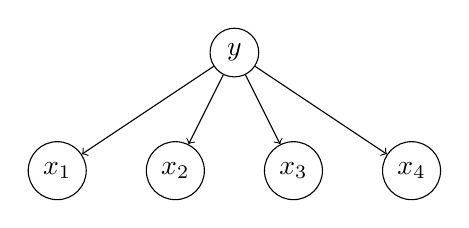
\begin{tikzpicture}[nodes={draw, circle}, ->]
        \node {$y$}
            child {node {$x_1$}}
            child {node {$x_2$}}
            child {node {$x_3$}}
            child {node {$x_4$}};
    \end{tikzpicture}
    \caption{Bayesian network with $4$ features representing the naïve Bayes classifier}
    \label{fig:my_label}
\end{figure}

Graphical models give us a graphical way to represent the joint PDF. It models the conditional dependencies between random variables. From this graph, we see that the joint probability distribution of this classifier is

\begin{equation*}
    p(y, x_1, x_2, x_3, x_4) = p(y)p(x_1|y)p(x_2|y)p(x_3|y)p(x_4|y)
\end{equation*}

\subsection{Naïve Bayes Classifier: Baseline Method}
\label{relatedwork:naiveBayes}
The naïve Bayes classifier is the simplest Bayesian network, assuming that all features are independent conditionally on the class variable, hence the name naïve Bayes. This naïve assumption gives the model few parameters to learn, and it requires little training data to achieve good performance. From the work by \citet{Zhang:2004:AAAI} we know that naïve Bayes classifiers perform well despite the assumption of independence among features due to the dependencies cancelling each other out and dependencies distributing evenly among classes.

According to \citet[p.~217]{Ankan:2015:Book}, assume that we have a dataset $X = (x_1, x_2, \dots, x_N)$ with $N$ independent features and $k$ classes $C_k$ that we want to classify the data to. naïve Bayes does this by modelling the posterior distribution in terms of the joint probability

$$
P(C_k | X) \propto P(C_k , X) = P(C_k) \prod_{i=1}^{n} P(x_i|C_k)
$$

Where the naïve assumption is that $P(x_i | X \setminus x_i , C_k) = P(x_i | C_k)$ i.e., the features are mutually independent conditioned on $C_k$. Different naïve Bayes methods exist for the assumptions on the priors and likelihoods, i.e. if they are Gaussian, binomial, categorical etc. The model classifies the data to the class that has the highest posterior probability. 

\subsection{pgmpy: naïve Bayes}

We have used the naïve Bayes classifier implemented in pgmpy and is used as a baseline method in the experiment described in section~\ref{sec:AdultFairnessAssessment}. The implementation in pgmpy implements a naïve Bayes method and assumes categorical distributions on all parameters. We calculated the probabilities as conditional probability tables (CPD Tables) using the MLE estimate from data. I.e. calculating probabilities from the dataset by counting occurrences conditioned on the class label. For more detail on how this is implemented, see pgmpy's documentation \footnote{\url{https://pgmpy.org/index.html}}.

\subsection{Structure Learning: Hill Climb Search}
\label{HillClimbSearch}
According to \citet[p.~811]{Koller:2009:Book} finding a maximum-score graphical network evaluated under any decomposable scoring function is NP-hard. Thus, we have to resort to a heuristic algorithm that attempt to find the best network, but are not guaranteed to do so. We have used Hill-Climb search which try to find the best graph $G_{\text{best}}$ by selecting an initial network $G_{\emptyset}$, which in pgmpy is a network with no edges. Then we search through all possible search operations $O$ to the network (delete, add, reverse in pgmpy) and score them. We perform the change that gives the best score until convergence or the maximum number of iterations is reached. The algorithm is shown below:

\begin{algorithm}
    \caption{Hill Climb Searched with Data Perturbation}
    \begin{algorithmic}
        \REQUIRE $G_{\emptyset} = $ Initial Network, $D = $ fully observed dataset, score $ = $ scoring function, $O = $ search operations, search $ = $ search procedure, $t_0 = $ initial perturbation size, $\gamma = $ Reduction in perturbation size.
        \ENSURE $G_{\text{best}} = $ Best network structure found.
        \STATE $G \leftarrow$ Search$(G_{\emptyset}, D, \text{Score}, O)$ 
        \STATE $G_{\text{best}} \leftarrow G$
        \STATE $t \leftarrow t_0$
        \FOR{$i \in \{ 1, \dots, \text{until convergence} \}$} 
        \STATE $D' \leftarrow $ Perturb$(D,t)$
        \STATE $G \leftarrow$ Search$(G, D', \text{Score}, O)$
        \IF{Score$(G : D) > \text{Score}(G_{\text{best}} : D)$}
            \STATE $G_{\text{best}} \leftarrow G$
        \ENDIF
        \STATE $t \leftarrow \gamma \cdot t$
        \ENDFOR
    \end{algorithmic}
\end{algorithm}

For more information about the algorithm and Hill Climb Search, see \cite[p.~816--819]{Koller:2009:Book} and the implementation in pgmpy which also adds some parameters like red-listed edges and non-changable edges.\footnote{\url{https:/Z/pgmpy.org/_modules/pgmpy/estimators/HillClimbSearch.html\#HillClimbSearch.estimate}}

\subsection{Parameter Learning: Expectation Maximization}
\label{Expectation Maximization}
After we have learned the model structure, we will have to learn the parameters of the model given its structure. Since we will use a model with latent variables, Expectation Maximisation is the algorithm of choice. The expectation maximisation algorithm in general as described by \citet{Murphy:2012:Book, Bishop:2006:Book} is as follows:

Consider a probabilistic model in which we collectively denote all the observed
variables by $\boldsymbol{X}$ and the latent variables $\boldsymbol{Z}$. The joint distribution $p(\boldsymbol{X}, \boldsymbol{Z} | \boldsymbol{\theta})$ is governed by the parameters $\boldsymbol{\theta}$. We want to maximise the likelihood given by

\begin{equation*}
    p(\boldsymbol{X} | \boldsymbol{\theta}) = \sum_{\boldsymbol{X}} p(\boldsymbol{X}, \boldsymbol{Z} | \boldsymbol{\theta})
\end{equation*}

Which is not computable, as $\boldsymbol{Z}$ is unknown. Therefore the expectation step is introduced which is to compute $Q$

\begin{equation*}
    Q(\boldsymbol{\theta, \theta^{\text{old}}}) = E[\log L(\boldsymbol{\theta}; \boldsymbol{X}, \boldsymbol{Z})]
\end{equation*}

In the M step we optimise $Q$ wrt $\boldsymbol{\theta}$

\begin{equation*}
    \boldsymbol{\theta^{\text{new}}} = \argmax_{\boldsymbol{\theta}} Q(\boldsymbol{\theta, \theta^{\text{old}}})
\end{equation*}

this is done iteratively until a certain threshold is achieved. For more details on how exactly this is implemented in pgmpy, see the documentation.\footnote{\url{https://pgmpy.org/_modules/pgmpy/estimators/EM.html\#ExpectationMaximization}}

\section{Modeling Discrimination Process}
\label{sec:paper1}
Now that probabilistic machine learning and graphical models have been introduced, it is time to introduce the work of \citet{Choi:2021:AIII} in more detail. As discussed previously in this section. There are many sources of bias in data and it is reasonable to assume that almost all datasets out there is biased. \citet{Choi:2021:AIII} describes a way of learning fair probability distributions from biased data by explicitly modeling a latent variable that represents a hidden, unbiased label. In particular, they aim to achieve demographic parity by enforcing
certain independencies in the learned model.

\begin{figure}[h!]
    \centering
    \begin{tikzpicture}[nodes={draw, circle}, ->]
        \node (S) {$S$};
        \node (Df) [right=of S] {$D_f$};
        \node (X)  [below=of S] {$X$};
        \node (D)  [below=of Df] {$D$};
        
        \draw (S) -> (X);
        \draw (S) -> (D);
        \draw (Df) -> (X);
        \draw (Df) -> (D);
    \end{tikzpicture}
    \caption{Bayesian network structures that represent the proposed
fair latent variable approach from \cite{Choi:2021:AIII}}
    \label{fig:choinetwork}
\end{figure}

In other words, they model the process on how biased datasets are generated. The biased labels present in the dataset are dependent on the sensitive attributes $S$ and the true fair labels $D_f$. The latent variable $D_f$ is used for decision making on future instances by inferring $P(D_f|e)$ given some evidence.

The paper states that any probabilistic model can be used but that this model needs to satisfy the independence assumptions in the Bayesian network.

\section{Fair Tree Classifier}
\label{sec:fairtree}

The paper by \citet{Antonio:2021:arXiv} has been implemented in this thesis and the related python module. They introduce a new splitting criterion that evaluates splits in terms of the Area under curve (AUC) wrt the predicted value and the sensitive attribute. Assume that we want to learn a classifier $f$ that learns a mapping from features $X$ and predictor $\hat{Y}$ which outputs a probability of belonging to the predicted class

$$
f: X \rightarrow \hat{Y}
$$

The AUC for this predictor wrt the true labels $Y$ can be calculated as

\begin{equation*}
    AUC_Y(\hat{Y}, Y) =  \frac
    {
        \sum_{t_0 \in Y_{-}} \sum_{t_1 \in Y_{+}}  \textbf{1}[\hat{Y}_{t_0} < \hat{Y}_{t_1}]
    }
    {
        |Y_{-}| \cdot |Y_{+}|
    }
\end{equation*}

where $Y_-$ and $Y_+$ are the set of indexes for negative and positive instances in the true labels. $\textbf{1}$ denotes the indicator function. The authors calculate the AUC score for the predicted labels this using scikit-learn \cite{Pedregosa:2011:JMLR} and the method called roc\_auc\_score \cite{Buitinck:2013:PKDD}. When calculating the AUC wrt the sensitive attribute, denoted $AUC_s$ the authors have derived the following formula

\begin{equation}
    AUC(\hat{Y}, S) = \max(1 - AUC(\hat{Y}, S), AUC(\hat{Y}, S))
\end{equation}

The max operator maps the bounds to the range $[0.5, 1]$. The authors then introduce the splitting criterion used in their tree algorihm, Splitting Criterion AUC for Fairness (SCAFF). Which is calculated as

\begin{equation*}
    SCAFF(\hat{Y}, Y, S, \Theta) = (1 - \Theta) \cdot AUC_Y(\hat{Y}, Y) - \Theta \cdot AUC_S(\hat{Y}, S)
\end{equation*}

$\Theta$ is here a hyperparameter of the tree classifier. When $\Theta = 1$ splits are only evaluated in terms of fairness and vice versa.  As is typical with tree learning, the architecture is learned by evaluating splits at each depth and selecting the split that maximises the splitting criterion. Other hyperparameters as maximum depth, number of bins etc are also used.

\section{Interpretable Machine Learning}

Up until this point in the thesis, we have discussed fair machine learning models and sources of bias in the data. Another important field in machine learning that is important regarding fairness is Interpretable Machine Learning. Many methods for fairness rely on either pre-processing of the datasets to make the datasets more fair or in-processing methods that change the machine learning algorithm to reduce discrimination during training. \cite{Mehrabi:2021:CSUR} 

Interpretable Machine Learning methods instead focus on understanding the mechanisms behind the decision that the machine learning model makes. This way, we can investigate how the machine learning model uses the data to make a prediction. According to \citet{Miller:2019:AIJ} interpretability is how well a human could understand the decisions in the given context. The higher the interpretability of a machine learning model, the easier it is for someone to comprehend why certain decisions or predictions have been made. \cite{Molnar:2020:Book}

\subsection{Example of interpretability}

Examples of interpretable machine learning models are Linear Regression, Logistic Regression and Decision Trees among many others. Linear Regression is especially interpretable, as we shall describe in this section. According to \citet{Molnar:2020:Book}, linear models can be used to model the dependence of a regression target $\boldsymbol{y}$ on some features $\boldsymbol{x}$. The learned relationships are linear and can be written for a single instance i as follows

\begin{equation*}
    \boldsymbol{y} = \boldsymbol{X} \boldsymbol{\beta} + \epsilon
\end{equation*}

Where $\beta_1$ is the weight associated with feature $X_1$. These weights can be interpreted in several ways depending on the nature of the feature.

\begin{itemize}
    \item Numerical Features: Increasing the feature by a unit of one increases the estimated outcome by $\beta_i$.
    \item Binary Feature: Changing the binary feature form the reference category to other category increases the outcome by $\beta_i$
    \item Categorical Feature: Create dummy variables. Interpretation of each dummy variable is the same as for binary features.
\end{itemize}

As you see, linear regression models are structured in such a way that it is easy to explicitly describe how the predictions of the models are made. Other models are also interpretable, which is described in more detail by \citet{Molnar:2020:Book}.
\chapter{Approach}
\label{ch:approach}

\section{Overall Approach}
To answer the three research questions mentioned in section~\ref{sec:intro:objectives} we want to compare some models find in literature. Mainly the fair Bayesian network and the fair tree classifiers. These should be evaluated on datasets used in machine learning research. We then will perform experiments evaluating the performance metrics of the models, as well as new performance metrics reflecting fairness. When we have enough data on the performance of the models, hypothesis testing will be done to evaluate whether the differences are significant.

\section{Python Code Repository: Forseti}

\begin{figure}
    \centering
    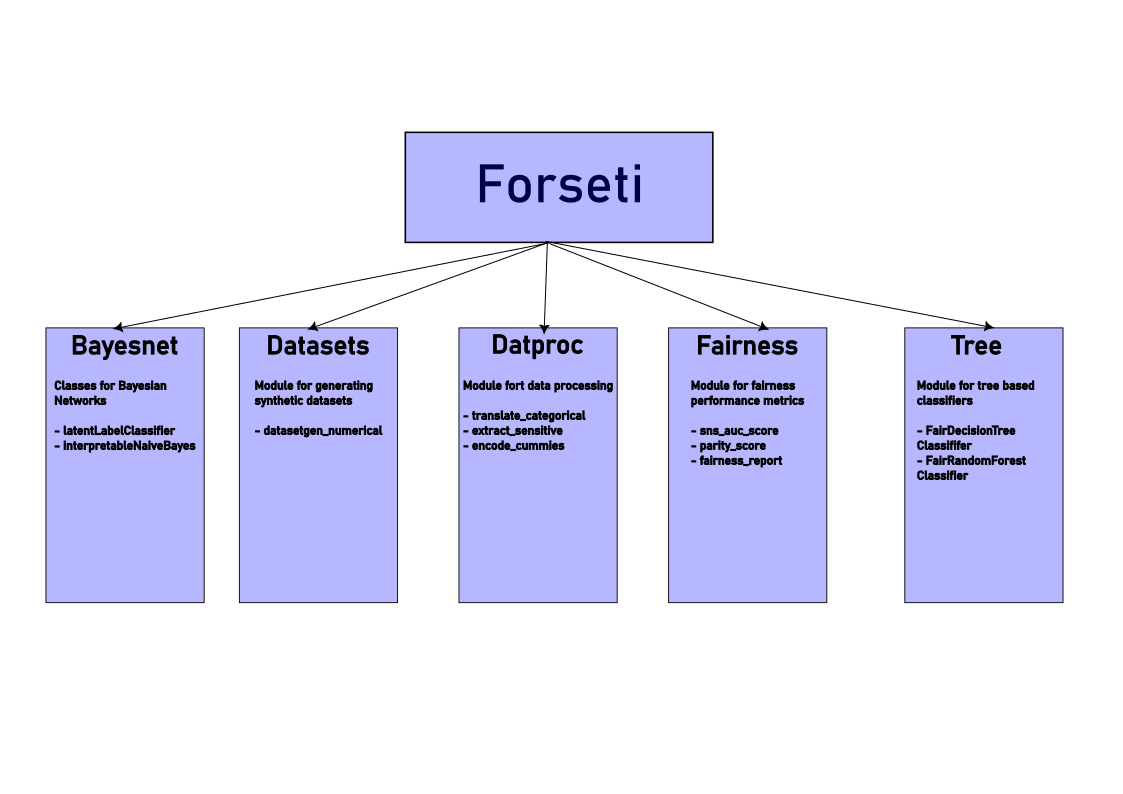
\includegraphics[width=\linewidth]{figures/tegning.png}
    \caption{Setup of Forseti Python Module}
    \label{fig:forseti}
\end{figure}

We manage the code through GitHub, a python module named Forseti as well as some Jupyter notebooks. In figure \ref{fig:forseti} the structure of the module is shown. It has the following modules:

\begin{itemize}
    \item Bayesnet: This module contains classes of Bayesian networks.
    \item Datasets: This module contains functions for generating synthetic datasets.
    \item Datproc: Data processing module.
    \item Fairness: Fairness metrics and fairness reports.
    \item Tree: Tree based methods and classifiers.
\end{itemize}

The code and its documentation is available at GitHub\footnote{\url{https://github.com/bcwein/forseti}}. The aim of organising the code in such a way was to make it as easy as possible to let others run the code on their own systems. How to do this is described in the next section.

\subsection{Setup}

The environment used in forseti is available in the file \emph{environment.yml} and one can setup the environment using Anaconda. See the documentation \footnote{\url{https://docs.conda.io/projects/conda/en/latest/user-guide/tasks/manage-environments.html\#creating-an-environment-from-an-environment-yml-file}} on how to do this.

If one prefers to not use anaconda, the necessary packages are as follows:

\begin{itemize}
    \item Python
    \item Pytest
    \item black
    \item jupyter
    \item ipykernel
    \item pandas
    \item seaborn
    \item pip
    \item pgmpy
\end{itemize}

\section{Data Exploration and Selection}

For this thesis, exploration of approaches to achieve fairness and interpretability in machine learning algorithms is the goal. The Adult dataset \footnote{\url{https://archive.ics.uci.edu/ml/datasets/adult}} was selected for this topic. Before beginning on implementing machine learning methods and experiments, some preliminary data exploration is in order.

\subsection{Adult Dataset}

To select the features of interest and as an initial data exploration. We will investigate the correlation between the features and the dependent variable \emph{income}. Since almost all the attributes are categorical, we calculate correlation using dummy variables. Which means, transforming categorical attributes to columns of binary attributes. We then explore which dummy variables that have the highest absolute correlations. We interpret the weight of each variable as the absolute sum of its dummies. 

\subsection{Compas Dataset}
The Compas dataset contains records for defendants from Broward County indicating their jail and prison times, demographics, criminal histories and Compas risk scores from 2013 to 2014 \cite{Mehrabi:2021:CSUR}. This dataset is high dimensional with a mix of categorical, numerical and date time columns. For this thesis, the focus has not been to implement the best model out there, but rather compare the fairness between models. Therefore, we have limited ourselves to the following attributes when training our algorithms

\begin{itemize}
    \item Sex: Gender of individual (binary)
    \item Age: Age of individual (positive integer)
    \item Race: Ethnicity of individual (6 categories)
    \item Priors Count: Prior Crimes (positive integer)
    \item Juvenile felony count: Felonies as a juvenile (positive integer)
    \item Juvenile misdemeanour count: Misdemeanours as a juvenile (positive integer)
    \item Juvenile other count: Other charges as a juvenile (positive integer)
    \item Charge degree: Degree of current charge (binary)
    \item Two year recidivism: Whether individual reoffended within two years (binary)
\end{itemize}

We selected these attributes mainly due to these being the only attributes in the dataset that are not recorded after rearrest and were not in a date time format. The point is not to make the best performing classifier, but to compare classifiers with regard to fairness.

\section{Metric for fair machine learning}

Using demographic parity as described in equation~\ref{eq:dempar} is the metric of choice for evaluating the model fairness in this thesis. The main reason for this is that the metric does not assume that the dataset labels are fair. Demographic parity is appropriate to use when we want our predictions to be more in line with a state of nature that we want to see in the world and when we are aware of historical biases that affect the data.~\footnote{\url{https://bit.ly/3Ko10sL}}. In the case of the adult dataset described in section~\ref{sec:adult}, we have the binary sensitive attributes \emph{gender} and the categorical sensitive attribute \emph{race}, both of which are known to experience discrimination in income. 

\begin{figure}
    \centering
    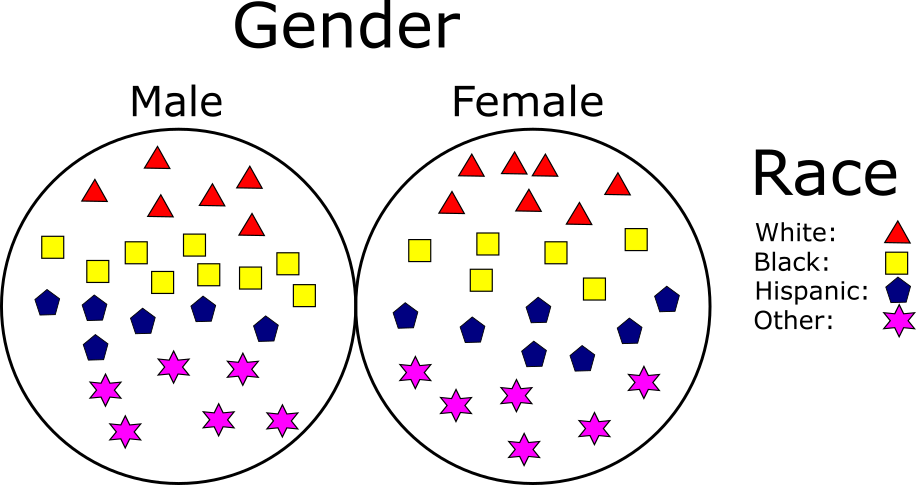
\includegraphics[width=0.7\linewidth]{figures/GroupOverlap.png}
    \caption{Visualisation of overlapping groups.}
    \label{fig:overlap}
\end{figure}

A challenge when working with multiple sensitive attributes and multivariate sensitive attributes is that you get overlapping groups. See figure~\ref{fig:overlap} for an example. There we see that we have the binary attribute \emph{Gender} and the categorical \emph{Race} we have several subgroups, i.e., Black Women, White Male etc. An algorithm can be \emph{independently group fair} when you calculate fairness for each sensitive attribute independently, and/or \emph{intersectional group fair} when you calculate fairness for all subgroups. \cite{Yang:2020:CoRR}. In this thesis, we use both approaches to calculate parity. 

\subsection{Scoring Function: Demographic Parity Score}
\label{sec:demparscore}
We defined a new scoring function based on demographic parity in equation~\ref{eq:dempar}, where $\hat{Y}$ is the predictor and $S$ the sensitive attribute. This equation can be generalised to the case where we have a categorical sensitive attribute with $K$ classes.

$$
P(\hat{Y} | S_i) = P(\hat{Y} | S_j) \qquad i, j \in \{0, \dots, K-1\}, \qquad i \neq j
$$

When calculating the probabilities, we want to condense these probabilities to a single metric between $0$ and $1$. I.e, when we have the likelihood of a positive outcome for the different classes of a sensitive attribute in a list of  probabilities $L$ like so

$$
L =\{ P(\hat{Y}=1 | S=0), \dots, P(\hat{Y}=1 | S=K-1) \}
$$

We want a function $f$ that takes such a list and maps it to a real number between $0$ and $1$

$$
f: L \rightarrow [0, 1]
$$

It is important that this function works for a list of likelihoods of arbitrary length, since we want to evaluate demographic parity for both binary and categorical sensitive attributes as well as all intersections of the sensitive attributes. Given the definition of demographic parity, we want the likelihoods to be as equal as possible. The scoring function derived is shown below

$$
f = 1 - 2\sigma(L)
$$

\begin{table}[]
    \centering
    \begin{tabular}{|l|l|}
        \hline
        $L$                 & $f$  \\ \hline
        {[}0.5, 0.5{]}      & 1    \\ \hline
        {[}0.6, 0.7{]}      & 0.9  \\ \hline
        {[}0.6, 0.8, 0.4{]} & 0.67 \\ \hline
        {[}0, 1, 0, 1{]}    & 0    \\ \hline
    \end{tabular}
    \caption{Example of values of $f$ given different lists of likelihoods.}
    \label{tab:scorefunc}
\end{table}

where $\sigma$ denotes the standard deviation. We plotted the scoring function in figure~\ref{fig:scorefunc}. The scoring function receives a list of two probabilities which slowly diverges from being equal at $0.5$ to the complete opposite, i.e $[0, 1]$. When the probabilities are equal, the score is 0 and if they are very different, the score is 0. See the examples of scores in table~\ref{tab:scorefunc}

\begin{figure}
    \centering
    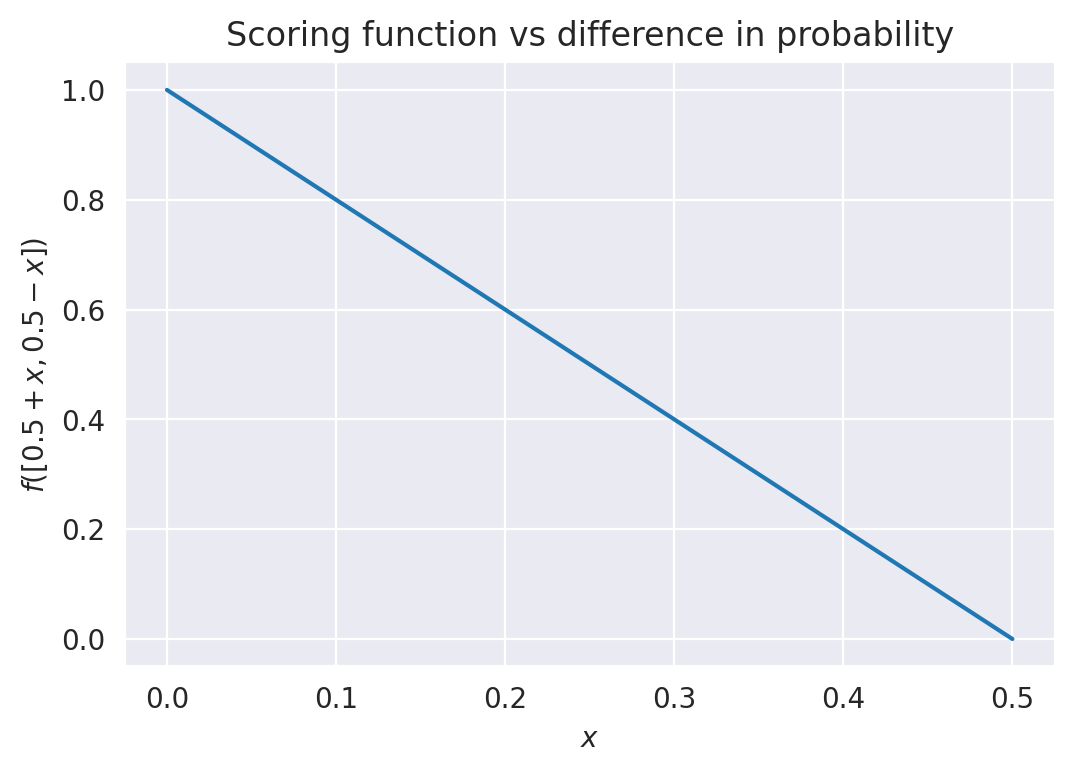
\includegraphics[width=0.7\linewidth]{figures/Parity_metric.png}
    \caption{Scoring function for a list of two diverging probabilities}
    \label{fig:scorefunc}
\end{figure}

\section{Fair Bayesian Network}
\label{sec:fairbayesiannetwork}
Based on the fair Bayesian network described by \citet{Choi:2021:AIII}, the following algorithm was derived.

\begin{algorithm}
    \caption{Latent Label Classifier Training}
    \begin{algorithmic}
        \REQUIRE $D = $ Training Dataset, $S = $ Sensitive Attributes, $L = $ attribute to predict. $t = $ tolerance for expectation maximisation.
        \ENSURE $M = $ Trained Bayesian network.
        \STATE Set of blacklisted nodes: $B = \{(x, y) \quad \forall x \in D.\text{columns}, \quad \forall y \in S\}$
        \STATE $M$.structure $=$ HillClimbSearch($D.$columns $\setminus L$, $B$)
        \STATE $M.$structure$ \cup \{ (x, L) \quad \forall x \in $S$\}$
        \STATE initialise fair node $F$
        \STATE $M.$structure$ \cup \{ (F, x) \quad \forall x \in D.\text{columns}\}$
        \STATE $M.$structure$ \cup \{ (F, L)\}$
        \STATE M.parameters $=$ ExpectationMaximisation($M$.structure, $D$)
        \RETURN M 
    \end{algorithmic}
\end{algorithm}

This method uses two methods implemented in pgmpy \cite{Ankan:2015:SCIPY}. These are Hill Climb Search for learning the structure which is described in section~\ref{HillClimbSearch} and Expectation Maximisation which is described in section~\ref{Expectation Maximization}. The resulting Bayesian network on the adult dataset is shown below in figure~\ref{fig:latentFairClassifierAdult}.

\begin{figure}[h!]
    \centering
    \begin{tikzpicture}[nodes={draw, circle}, ->]
        \node (Race) {$R$};
        \node (Gender) [right=of Race]{$G$};
        \node (Fair) [right=of Gender] {$F$};
        \node (Capital) [below=2cm of Race] {$C$};
        \node (Relationship) [left=of Capital] {$R_e$};
        \node (Education) [left=of Relationship] {$E$};
        \node (Age) [left=of Education] {$A$};
        \node (Marital) [right=of Capital] {$M$};
        \node (Workclass) [right=of Marital] {$W$};
        \node (Hours) [right=of Workclass] {$H$};
        \node (Occupation) [right=of Hours] {$O$};
        \node (Income) [right=of Occupation] {$I$};

        \draw (Fair) -> (Age);
        \draw (Fair) -> (Education);
        \draw (Fair) -> (Relationship);
        \draw (Fair) -> (Capital);
        \draw (Fair) -> (Marital);
        \draw (Fair) -> (Workclass);
        \draw (Fair) -> (Hours);
        \draw (Fair) -> (Occupation);
        \draw (Fair) -> (Income);
        
        \draw (Race) -> (Income);
        \draw (Race) -> (Marital);
        
        \draw (Gender) -> (Relationship);
        \draw (Gender) -> (Marital);
        \draw (Gender) -> (Workclass);
        \draw (Gender) -> (Hours);
        \draw (Gender) -> (Occupation);
        \draw (Gender) -> (Income);
        
        \draw (Age) to  [out=270,in=240] (Hours);
        \draw (Relationship) to  [out=270,in=300] (Age);
        \draw (Relationship) to  [out=270,in=240] (Hours);
        \draw (Marital) to [out=270,in=300] (Age);
        \draw (Marital) to [out=270,in=300] (Relationship);
        \draw (Workclass) to [out=270,in=240] (Occupation);
        \draw (Hours) to [out=270,in=300] (Workclass);
        \draw (Hours) to [out=270,in=240] (Occupation);
        \draw (Occupation) to [out=270, in=300] (Education);
    \end{tikzpicture}
    \caption{latentFairClassifier trained on Adult Dataset. The nodes are $R$: race, $G$: gender, $F$: latent fair labels, $A$: Age, $E$: Education, $R_e$: Relationship, $C$: Capital gain, $M$: Marital Status, $W$: Work class, $H$: Hours-per-week, $O$: Occupation and $I$: Income.}
    \label{fig:latentFairClassifierAdult}
\end{figure}
Inference has been performed by evaluating $P(F | A, E, R_e, C, M, W, H, O)$ on a test dataset of unobserved labels.

\section{Fair Tree Classifier}
The fair tree classifier, described in detail in section~\ref{sec:fairtree}. \citet{Antonio:2021:arXiv} kindly provided their code on GitHub, which made implementing this over to Forseti a bit easier. The code is available in their repository\footnote{\url{https://bit.ly/3x937Nr}}. We added their decision tree classifier and fair random forest classifier classes to Forseti and train and test the models on the same datasets as the fair tree classifier.

\section{Experiment 1: Test Models on Compas and Adult Dataset}

After implementing the Fair Bayesian Network and the Fair Tree Classifier. We wanted to evaluate the models on the Adult Dataset and Compas Dataset. To evaluate the models we had to choose some performance metrics. A combination of traditional performance metrics and a fairness score was desired. The fairness score used is the one described in section~\ref{sec:demparscore}. For the traditional metrics there were several pros and cons for each of them. We will go through each one of them and explain the motivation for using that particular scoring method.

\subsection{Accuracy}

We use the accuracy score as implemented in Scikit Learn. Which follows the following formula

\begin{equation*}
    A(y, \hat{y}) = \frac{1}{n_\text{samples}} \sum_{i=0}^{n_\text{samples} - 1} 1(\hat{y}_i = y_i)
\end{equation*}

Accuracy is a very intuitive coring function for predictions, as it can be interpreted as the ratio of correct classifications. The problem with accuracy as a scoring function is when datasets are imbalanced, the scoring function also suffers and are biased toward the most prominent class.

\subsection{Balanced Accuracy}

Balanced Accuracy is calculated as follows

\begin{equation*}
    BA(y, \hat{y}) = \frac{1}{\sum \hat{w}_i} \sum_i 1(\hat{y}_i = y_i)\hat{w}_i
\end{equation*}

where $\hat{w}_i$ is sample weight of the i-th sample and the weight is adjusted to 

\begin{equation*}
    \hat{w}_i = \frac{w_i}{\sum_j 1(y_j = y_i)w_j}
\end{equation*}

Balanced Accuracy is equal to the arithmetic mean of the sensitivity and specificity in the binary case. Since this accuracy score scales with imbalanced datasets it gives a more clear picture of how well the classifier performs and adjusts if the classifier takes advantage of the imbalance.

\subsection{F1 Score}

The F1 score is defined as the harmonic mean of precision and recall and thus reflect. We chose to add F1 score as it is a commonly used score in machine learning and the score reflects how well the model is able to maximise precision and recall and not have a huge disparity between them. One challenge with F1 score is that it ignores true negatives. 

\subsection{Specificity}

And lastly, we calculate the specificity (true negative rate). Which is calculated from the confusion matrix as follows

\begin{equation*}
    TNR(\hat{y}, y) = \frac{TN}{N}
\end{equation*}

We mainly chose this metric since F1 score ignores true negatives and by having this in our fairness report we have some information with regard to true negatives.

\subsection{ROC Curve}

We also want to calculate the ROC curve and plot it to see the threshold independent performance of the model. This requires us to also get the predicted probability of positive outcome for the models. When we have the predicted probabilities and the true class labels. We use the different probability scores as thresholds, sort them and calculate the TPR and FPR for each probability score and plot TPR with FPR to produce the ROC curve. We use the method \emph{plot\_roc\_curve} in sklearn.

\subsection{Model Selection}

For the first experiment, we also want to compare our fair models with some baseline models. Additionally, we want to explore the hyperparameter-space of models that have hyperparameters. This led us to the following models to evaluate

\begin{itemize}
    \item \emph{FairBN}: Training a Fair Bayesian Network and doing inference on the latent fair variable.
    \item  \emph{IncomeBN}: Same model as FairBN. prediction is done on the variable Income instead of the latent fair attribute.
    \item \emph{NBSens} is a naïve Bayes classifier trained on all of the attributes available.
    \item \emph{NB} is a naïve Bayes classifier trained on the dataset without the sensitive attributes.
    \item \emph{FRFC03}: Fair Random Forest classifier with $\Theta = 0.3$
    \item \emph{FRFC05}: Fair Random Forest classifier with $\Theta = 0.5$
    \item \emph{FRFC07}: Fair Random Forest classifier with $\Theta = 0.7$
\end{itemize}

naïve Bayes with and without serves as the baseline method. Removing the sensitive attributes serves as a first attempt at achieving fairness by not allowing the model to explicitly use the sensitive attributes for prediction. We expect to see that the fair machine learning methods performs better in regard to fairness to the naïve Bayes model. Otherwise, there is no reason to use the fair methods. The results of the first experiment are shown in section~\ref{sec:result:experiment1}.

\section{Experiment 2: Performance on synthetic dataset and comparison of performance metrics.}

\subsection{Motivation for experiment}

The results in the first experiment shed some light on the challenge of calculating fairness. The fair Bayesian network classifier got higher parity scores as expected but for the random forest classifier, unexplained behaviour of the model with respect to the hyperparameter was observed. Since the parity score used in this experiment is a new and self proposed metric of fairness, this should be investigated further to evaluate its validity.

\citet{Antonio:2021:arXiv} claim that they have made a classifier able to give more fair predictions, and using a hyperparameter $\Theta$ that give more accurate predictions when $\Theta \rightarrow 0$ and more fair predictions when $\Theta \rightarrow 1$. We fail to reproduce these results when calculating parity score for the models. The authors themselves do not calculate intersectional parity score, but rather $AUC_S$ with respect to the individual sensitive attributes. Due to these observations, we chose to focus on how to calculate fairness and what are the limitations of the respective fairness metrics for the next iteration of experiments.

The two models that have been implemented in the first round of experiments, namely the fair Bayesian network introduced by and the Fair Tree Classifier introduced by. These classifiers have two different ways of evaluating fairness that is the motivation behind their design. In the work of \citet{Choi:2021:AIII} the model was designed in terms of demographic parity by modelling a Bayesian network in such a way that the sensitive attributes are independent of the predictions but still used for learning the parameters of the distribution of fair labels. In the work of \citet{Antonio:2021:arXiv} they use strong demographic parity as motivation for their model. They implement a tree based method where splits are evaluated using the threshold-independent measure of AUC with respect to the labels of the dataset and  regularised using AUC with respect to the sensitive attributes. 

\subsection{Experiment Design}

There are some question that have arisen from the first round of experiments and some improvements that we wanted to implement. These are

\begin{enumerate}
    \item Does demographic parity score capture fairness? \label{ex2:parityscore}
    \item What other measures of fairness can we introduce that are more well established? \label{ex2:fairnessmeasure}
    \item How does the different performance metrics used by the different authors compare?
    \item Collect enough samples to perform hypothesis testing.
\end{enumerate}

\subsection{Generating Synthetic Data}

To address question~\ref{ex2:parityscore}, we wanted to generate a synthetic dataset where we are in control of the bias in the data to see how the fairness measures fares. We implemented an algorithm for generating synthetic datasets with numerical (Gaussian) features as well as two sensitive features, gender, and race. The dataset can be either informative or non-informative. If the dataset is informative, the features are dependent on the sensitive attributes. I.e., there is bias in the data with respect to the sensitive attributes. We generate the dataset in the following way. The first attribute, gender $G_s$, is assumed to follow a Bernoulli distribution

\begin{equation*}
    G_s \sim B(n, p)
\end{equation*}

where $n = 1$ and $p = 0.5$. I.e. we assume that it is equally likely to be a male or female. The second attribute, Race $R_s$ is assumed to follow a categorical distribution 

\begin{equation*}
    R_s \sim C(k, \boldsymbol{\theta})
\end{equation*}

Which has PMF

\begin{equation*}
    f_{R_s}(R_s = i) = \boldsymbol{\theta}_i, \qquad i \in \{ 1, \dots, k\}
\end{equation*}

where $\boldsymbol{\theta}$ is a vector of $k$ event probabilities $p_i$. $(p_i \geq 0, \sum p_i = 1)$. We want to initialise $\boldsymbol{\theta}$ randomly and this is done by sampling $k$ numbers from $\tau$ which follows the standard half-normal distribution

\begin{equation*}
    \tau \sim |N(0, 1)|
\end{equation*}

And $\boldsymbol{\theta}$ is then calculated by arranging the $k$ samples from $\tau$ in a vector and transforming them to probabilities 

\begin{equation*}
    \boldsymbol{\theta} = ({\tau_1, \dots, \tau_k}) \cdot \frac{1}{\sum \tau}
\end{equation*}

The numerical values of the sensitive attributes are mapped to strings using a dictionary in python. Now that the sensitive attributes are sampled, we will sample the non-sensitive features. To simulate the discrimination process, we sample the features from Gaussian distributions that depend on the sensitive attributes. There are 4 numerical features where the first two depend on the gender and the last two depend on the race. Let's denote these features $X_1, X_2, X_3$ and $X_4$.

\begin{figure}
    \centering
    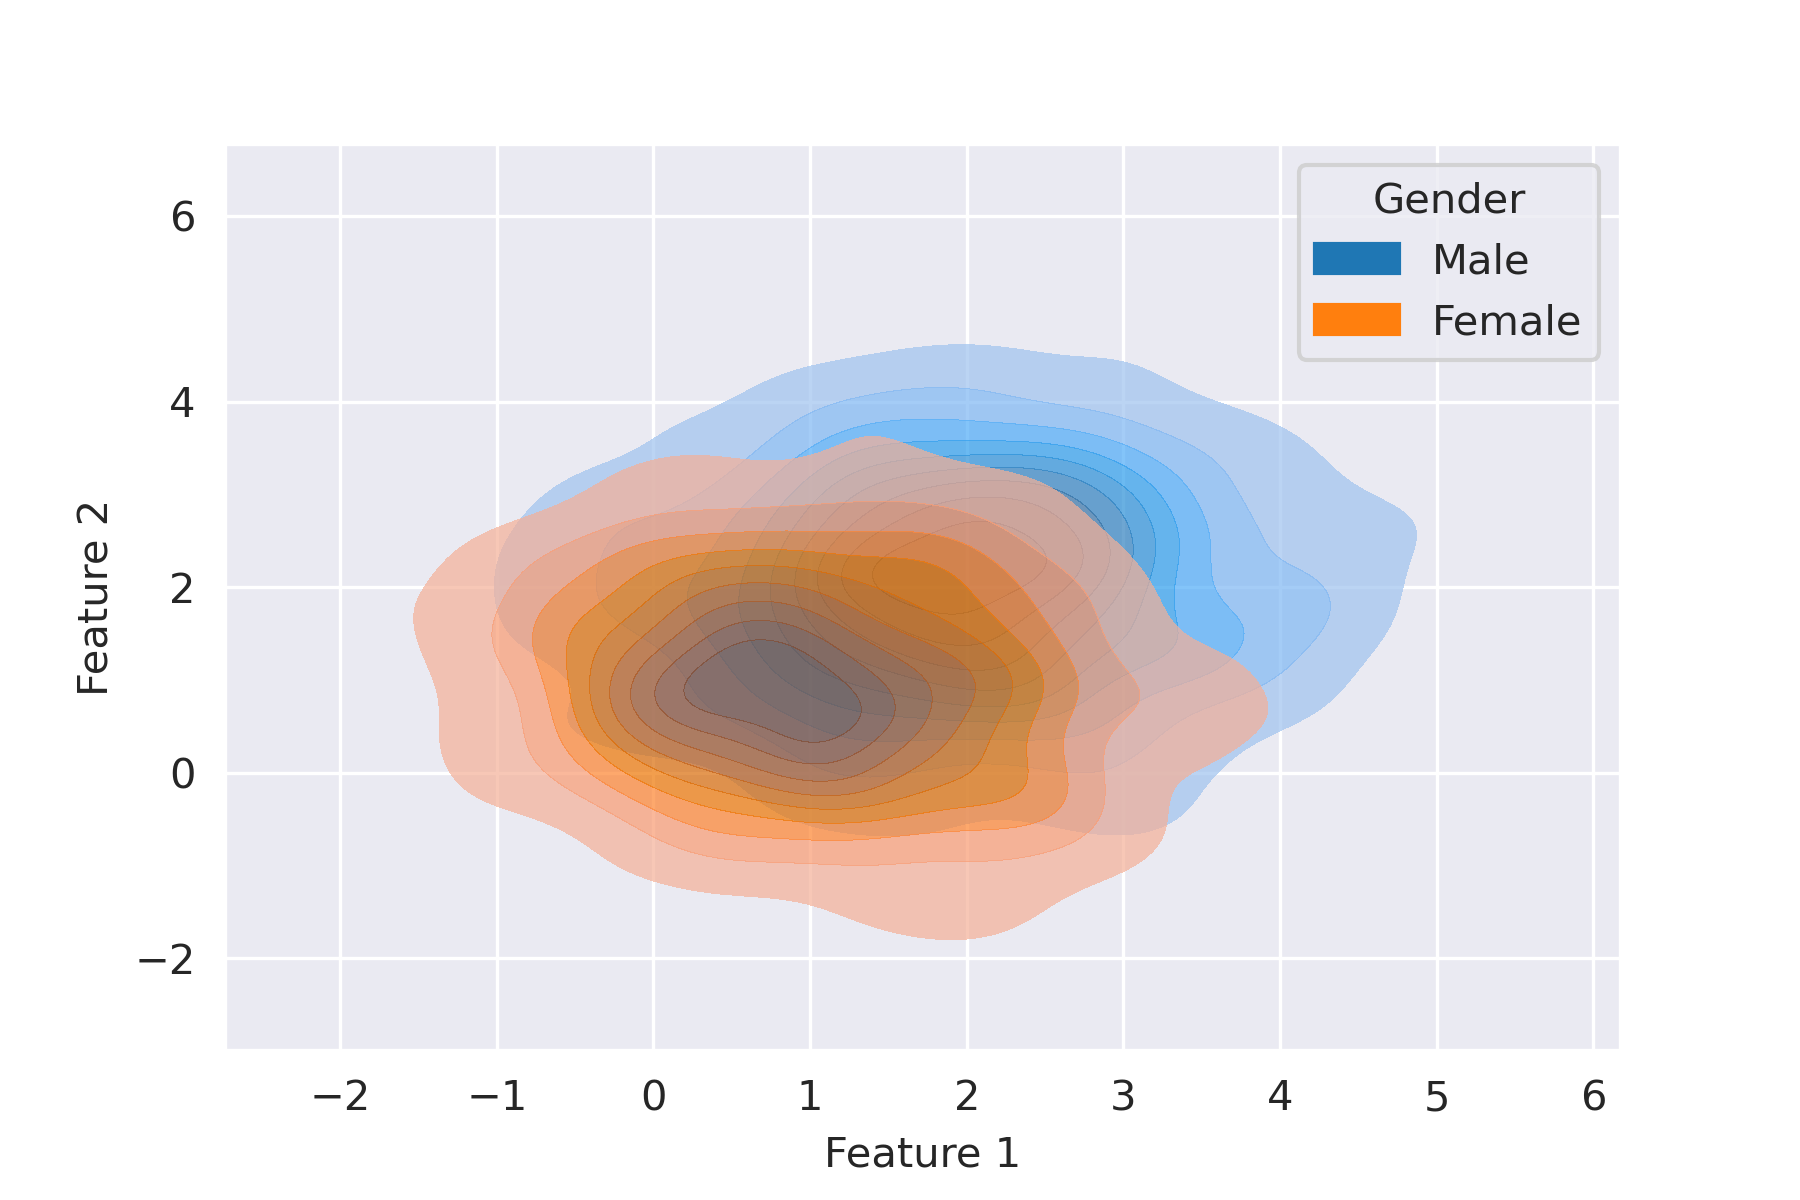
\includegraphics[width=0.49\linewidth]{figures/synthetic-gender.png}
    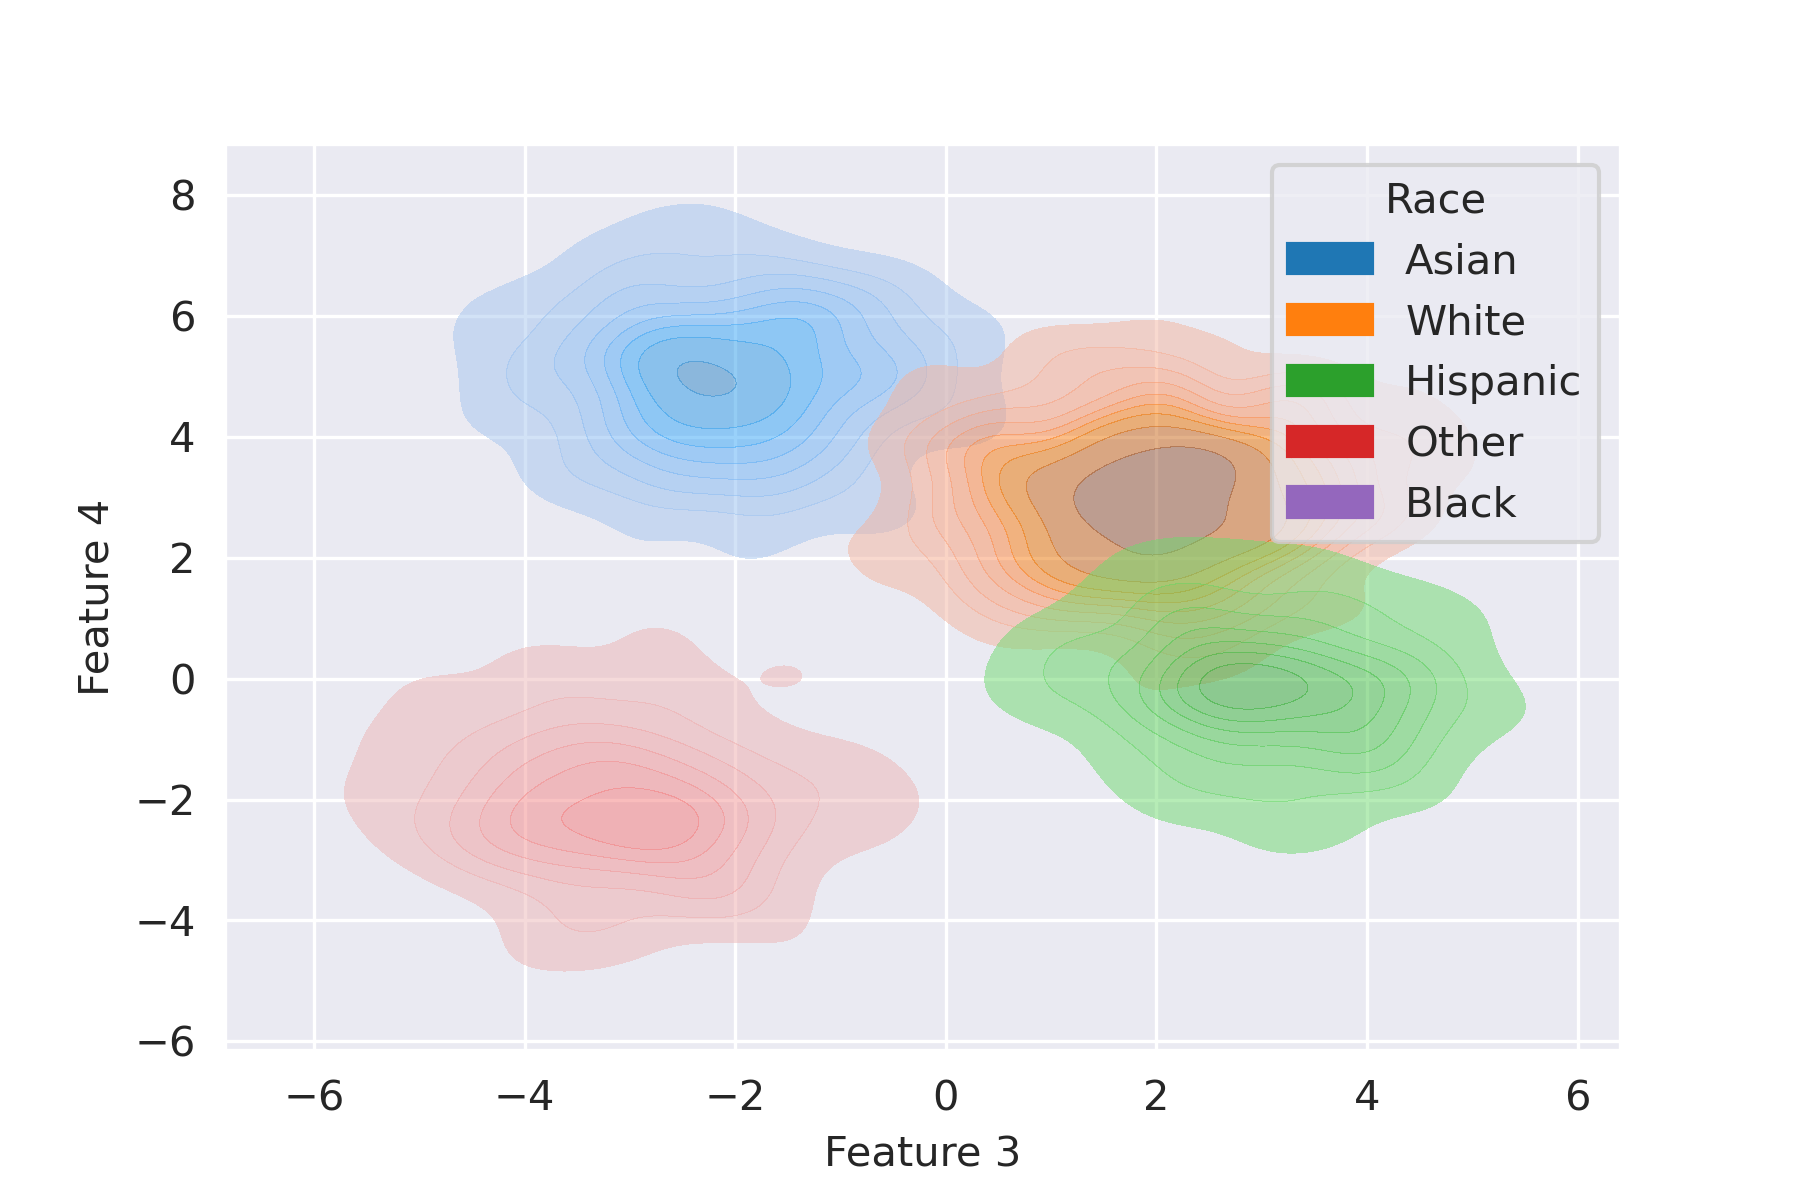
\includegraphics[width=0.49\linewidth]{figures/synthetic-race.png}
    \caption{KDE of the bivariate features of the synthetic dataset..}
    \label{fig:synthdatasetfeatures}
\end{figure}


We define a separator parameter $\Theta$ which is used to model the separation between the sensitive classes. We sample $X_1$ and $X_2$ the following way conditionally on the sensitive attribute $G_s$

\begin{equation*}
    \begin{aligned}
           X_1 | G_s = \text{Female} \sim N(1, 1) \\ 
           X_1 | G_s = \text{Male} \sim N(1 + \Theta, 1)
    \end{aligned}
\end{equation*}

And the same for $X_2$. The same principle is used for $X_3$ and $X_4$ but with a slight twist. There are $k$ races in the dataset and a random sign variable $R$ following the discrete uniform distribution over the set $\{-1, 1\}$.

\begin{equation*}
    \begin{aligned}
        X_3 | R_s = k \sim N(1 + \Theta \cdot R \cdot k, 1)
    \end{aligned}
\end{equation*}

and the same for $X_4$. Then lastly, to calculate the labels of the dataset we take the sum of all the numerical features $X = \{ X_1, X_2, X_3, X_4 \}$ and calculate the median of all the sums for each data point. If the sum is above the median, it gets labeled 1, otherwise, 0.

This can be summarised in algorithm~\ref{alg:datasetgen}

\begin{algorithm}
    \caption{Synthetic dataset generation}
    \begin{algorithmic}
        \REQUIRE $I = $ Informative. True or false, $\Theta = $ Separability, $N =$ Number of samples.
        \ENSURE $D = $ Synthetic Dataset.
        \STATE Sample $N$ samples from $G_s \sim B(1, 0.5)$
        \STATE $k = 5$
        \STATE $\boldsymbol{\tau_k} = \{ \tau_1, \dots, \tau_k \}$ with $\tau_j \sim |N(0, 1)|$
        \STATE $\theta = \boldsymbol{\tau} \cdot \frac{1}{\sum \tau_k}$
        \STATE Sample $N$ samples from $R_s \sim C(k, \theta)$
        \STATE Sample $N_{\text{Female}}$ samples from $X_1 \sim N(1, 1)$
        \STATE Sample $N_{\text{Male}}$ samples from $X_1 \sim N(1 + \Theta, 1)$
        \STATE Sample $N_{\text{Female}}$ samples from $X_2 \sim N(1, 1)$
        \STATE Sample $N_{\text{Male}}$ samples from $X_2 \sim N(1 + \Theta, 1)$
        \FORALL{$i \in \{ 1, \dots, k \}$}
        \STATE Select $R$ uniformly from the set $\{ -1, 1\}$
        \STATE Sample $N_i$ samples from $X_3 | R_s = i \sim N(1 + \Theta \cdot R \cdot i, 1)$
        \STATE Select $R$ uniformly from the set $\{ -1, 1\}$
        \STATE Sample $N_i$ samples from $X_4 | R_s = i \sim N(1 + \Theta \cdot R \cdot i, 1)$
        \ENDFOR
        \STATE $t = \sum X$ for all datapoints in the dataset
        \IF{$t \geq \text{Median}(X)$}
        \STATE $Y = 1$
        \ELSE
        \STATE $Y = 0$
        \ENDIF
        \STATE $D = \{G_s, R_s, X_1, X_2, X_3, X_4, Y \}$
        \RETURN $D$
    \end{algorithmic}
    \label{alg:datasetgen}
\end{algorithm}

\subsection{Fairness Performance Measure}

The performance metric used for the models up to this points is the parity score metric as described in Section.~\ref{sec:demparscore}. This score is based on the notion that the likelihood of positive outcome is independent of the sensitive attributes. There is another measure that is similar to this. That is Kullback-Leibler divergence. Which according to \citet{Mackay:2003:information} is calculated as 

\begin{equation*}
    D_KL(P ||Q) = \sum_x \log\frac{P(x)}{Q(x)}
\end{equation*}

Kullback-Leibler divergence is a measure of how different two distributions $P$ and $Q$ are. It is not strictly a metric as it is not symmetric and is instead a divergence. While metrics are symmetric and linear in distance, divergences are asymmetric and generalise square distance. For our work, we want to use Kullback-Leibler divergence as a measure of unfairness. The general idea is that we want $P$ and $Q$ to denote different distributions conditional on sensitive attributes. Assume that we have a dataset with model predictions $Y$ and a binary sensitive attribute $S$. Then we define 

\begin{equation*}
    P \sim Y | S = 0
\end{equation*}

and

\begin{equation*}
    Q \sim Y | S = 1
\end{equation*}

Under demographic parity, we want $Q \perp\!\!\!\perp P , S$ and thus a Kullback-Leibler Divergence of 0. Kullback-Leibler Divergence is limited to two distributions though there are generalisations. For this round of experiments we limit ourselves to the binary case and calculate the divergence in the binary cases and compare them to the other metrics.

\subsection{Hypothesis Tests}

We want to perform hypothesis testing on the performance metrics of different models. Assume that we have samples of an unspecified performance metric for two different models trained on the same dataset. Let us denote the two distributions $X$ and $Y$. 

We have chosen to use non-parametric hypothesis tests, as we do not want to make assumptions on the kind of distribution the samples have. Since the samples are of model performance of two machine learning models trained on the same dataset, the samples will be dependent on each other. We therefore select the Wilcoxon signed-rank test as the testing method of choice. This test was introduced and named after \citet{Wilcoxon:1945:Biometrics}. The Wilcoxon signed-ranked test calculates the differences between the ranked samples and test whether or not the differences are symmetric around zero. We will test the following hypotheses, shown in table~\ref{tab:hypothesis}.

\begin{table}
    \centering
    \begin{tabular}{p{10cm}lll}
        \hline
        \textbf{Hypothesis} & $\boldsymbol{H_0}$ & $\boldsymbol{H_1}$ & $\boldsymbol{\alpha}$ \\
        \hline
        \hline
        FairBN ($Y$) has a better intersectional parity score than naïve Bayes ($X$) without sensitive attributes & $X = Y$ & $X < Y$ & $0.01$ \\ \hline
        FRFC ($Y$) has a better intersectional parity score than naïve Bayes ($X$) without sensitive attributes & $X = Y$ & $X < Y$ & $0.01$ \\ \hline
        FairBN ($Y$) has a better intersectional parity score than FRFC ($X$) & $X = Y$ & $X < Y$ & $0.01$ \\ \hline
        FairBN ($Y$) has a better KLD w.r.t. Gender than FRFC ($X$) & $X = Y$ & $X > Y$ & $0.05$ \\ \hline
    \end{tabular}
    \caption{List of hypothesis}
    \label{tab:hypothesis}
\end{table}

\subsection{Experiment Setup}

We ran 100 synthetic dataset generations and trained the models on the synthetic datasets and evaluate them on a test dataset. For each iteration the train-test split is $70\%$ for the training set and $30\%$ for the test dataset. We calculated the same performance metrics as in the first experiment. Additionally, we also introduce Kullback-Leibler Divergence w.r.t. Gender. 

After the performance metrics have been calculated and collected. We will visualise the distributions of the performance metrics as well as the correlation between parity score, KL Divergence and AUC score. The results are shown and discussed in section~\ref{eval:exp2}

\section{Experiment 3: Interpretable Machine Learning}

We have been able to show that the models we have trained are able to satisfy some mathematical notion of fairness in their predictions. But we want to investigate this further. By employing interpretable machine learning methods, we can try to explain how the model uses the sensitive attributes in their predictions and try to explain their behaviour. 

\subsection{Experiment Design}

For this experiment, we want to implement the following in an attempt to explain the decisions made by machine learning models

\begin{itemize}
    \item Train a baseline interpretable model and investigate the decision rules it learns.
    \item Interpret the models that are interpretable by default.
    \item Use model agnostic interpretable methods for models that are not interpretable.
\end{itemize}

In the following sections, we will describe the methods chosen to answer the above points.

\subsection{Interpreting Decision Trees}

To address the first point, we want to train a baseline interpretable model. Our choice landed on Decision Trees. According to \citet{Molnar:2020:Book} the interpretation of decision trees, while quite similar for all algorithms, differ by the kind of algorithm for building the tree is used. The interpretation described here is for the CART algorithm, which is the one implemented by Scikit-learn \cite{Pedregosa:2011:JMLR}.

The interpretation of decision trees works as follows: Starting from the root node, you go to the next nodes and the edges tell you which subsets you are looking at. Once you reach the leaf node, the node tells you the predicted outcome. \cite{Molnar:2020:Book} To calculate the feature importance. We calculate the reduction in the split. In our case, we have used entropy and information gain to evaluate splits which is defined as 

\begin{equation*}
    IG(T) = H(T) - \sum_{i = 1}^{2} \frac{n_i}{n} H(C_i)
\end{equation*}

Where $T$ is the node being split and $C_i$ is child node $i$. $H$ denotes shannon entropy introduced by \citet{Shannon:1948:BellSystTechJ}. Go through all the splits for which the feature was used and measure how much it has reduced the information gain. Scale all the sums to $1$, then you can calculate the share of a features importance as an percentage.

We will do this for the datasets that have been used in the previous experiments to uncover what attributes are used in the model prediction.

\subsection{Interpreting naïve Bayes}

As described in section~\ref{relatedwork:naïvebayes}, the naïve Bayes classifier assumes that all features are mutually independent, conditioned on the class labels. We can therefore interpret the contributions of the different attributes through the conditional probabilities that the naïve Bayes classifier has learned \cite[p.~142]{Molnar:2020:Book}.

The way we have chosen to do this is like so: Assume that a feature $X_i$ in a dataset $\boldsymbol{X}$ is informative. Then we would expect that the likelihood on $X_i$ is very different given the class $Y$

\begin{equation*}
    P(X_i | Y = 0) \neq P(X_i | Y = 1)
\end{equation*}

In the case that $X_i$ is categorical with $k$ categories. We have a conditional dependency table on the form

\begin{equation*}
    \begin{bmatrix}
        P(X_0 | Y = 0) & P(X_0 | Y = 1) \\ 
        P(X_1 | Y = 0) & P(X_1 | Y = 1) \\
        \vdots & \vdots \\
        P(X_k | Y = 0) & P(X_k | Y = 0)
    \end{bmatrix}
\end{equation*}

Then we denote the first column $P = P(X_i | Y = 0)$ and the second column $Q = P(X_i | Y = 1)$. We assume that the more informative $X_i$ is as a feature, the difference in these distributions should increase. To calculate the feature weight we define the weight as 

\begin{equation*}
    D_{KL}(P||Q)
\end{equation*}

This should also be validated using permutation importance to compare the weights. Introduced by \ref{alg:permimp} is used and is based on the one used by Scikit-learn \cite{Pedregosa:2011:JMLR}

\begin{algorithm}
    \caption{Permutation Importance Algorithm}
    \begin{algorithmic}
        \REQUIRE $C = $ Classifier, $D = $ Test Dataset. $K = $ No of permutations.
        \ENSURE $I = $ Dataset of importances.
        \STATE Compute reference score $S$ on the test dataset $D$.
        \FORALL{columns $i\in D$}
            \FOR{$j \in \{ 1, \dots, K \}$} 
                \STATE Permute (shuffle) column $D_{i}$ and denote the corrupted dataset $\Tilde{D}_{j}$
                \STATE Compute score $s_{ij}$ on test dataset $\Tilde{D}_{j}$
                \STATE Set $I_{ij} = S - s_{ij}$
            \ENDFOR
        \ENDFOR
        \RETURN $I$ 
    \end{algorithmic}
    \label{alg:permimp}
\end{algorithm}

This algorithm returns a dataset of importances, as we want to see the distribution of importances for each feature.

\subsection{Interpreting Bayesian Networks}

Bayesian Networks are to some extent interpretable machine learning models, dependent on the complexity of the conditional dependencies. Naïve Bayes is an interpretable machine learning model and is the simplest Bayesian network. It is very intuitive for humans to explain how much each attribute contributes, as they are conditionally independent given the class label. As the complexity of the conditional dependencies increase,  they are more demanding to understand.

In our case, from the fair Bayesian network as shown in figure \ref{fig:choinetwork}. We see that the sensitive attributes are independent of the true latent dataset labels. Meaning that the sensitive attributes should not be used explicitly in the prediction. To investigate this, we want to use the permutation importance algorithm to see how important the features are for getting accurate predictions. We will also apply counterfactual generation described in section~\ref{sec:counterfactuals} on the fair Bayesian network for further interpretability.

\subsection{Interpreting Fair Random Forest}

Random Forests are not interpretable as the many different trees used for predictions are not immediately intuitive to explain, and in many cases so many that the interpretation is incomprehensible in human terms. Therefore, one has to resort to model agnostic interpretability methods if one wants to gain some insight. We have chosen to use feature importance here as well in an effort to understand the model.

There is one challenge with the approach by \citet{Antonio:2021:arXiv}, and that is the fact that the sensitive attributes are only used during training of the model. Meaning that one cannot infer how the model uses the sensitive attributes neither using the permutation importance method nor counterfactual generation. We will resort to investigate how the model uses the non-sensitive attributes in their prediction to investigate how the model achieves fairness.

\subsection{Counterfactuals}
\label{sec:counterfactuals}

According to \citet{Molnar:2020:Book}, a counterfactual explanation should describe the smallest change to the feature values that changes the prediction to a predefined output. In our case for the Adult and the Compas dataset, we want to generate the smallest changes to get a positive outcome (being classified as high income or not likely to reoffend). Counterfactuals should follow these criteria

\begin{itemize}
    \item Counterfactuals should be as similar as possible to the instance regarding feature values.
    \item Counterfactual instances should have feature values that are likely.
    \item Change as few features as possible.
\end{itemize}

Various methods exist for generating counterfactuals, while we will get inspiration from the method proposed by \citet{Dandl:2020:PPSN}, specifically the NSGA-II algorithm introduced by \citet{Pratap:2002:IEEE.Trans.Evol.Comput.}. We want to generate counterfactuals that satisfy the following objectives 

\begin{equation*}
    o_1(\hat{f}(\boldsymbol{x}), Y') = 
    \begin{cases}
        0 & \text{if} \hat{f}(\boldsymbol{x}) \in Y' \\
        \underset{y' \in Y'}{\text{inf}} |\hat{f}(\boldsymbol{x}) - y'0|, & \text{else} \\
    \end{cases}
\end{equation*}

Which is the distance between the desired prediction $y'$ and the predicted value $\hat{f}(\boldsymbol{x})$.  The second objetive $o_2$ reflect that counterfactuals should be as equal to the instance $\boldsymbol{x}$ that we want to flip the prediction for

\begin{equation*}
    o_2(\boldsymbol{x}, \boldsymbol{x'}) = \frac{1}{p} \sum_{j=1}^{p} \mathbb{I}_{x_j \neq x'_j}
 \end{equation*}

Which uses the indicator function,  as the models implemented in pgmpy uses categorical data. Numerical values are also categorical as they are discretised. Next, we introduce $o_3$ which measures the amount of features that have been changes.

\begin{equation*}
    o_3(\boldsymbol{x}, \boldsymbol{x'}) = ||\boldsymbol{x} - \boldsymbol{x'}||_0 = \sum_{j=1}^{p} \mathbb{I}_{x_j \neq x'_j}
\end{equation*}

Lastly, we want the counterfactual to have attributes that are likely to occur. We measure this by searching for the closest sample in the training dataset and calculate the distance between the candidate and the closest point.

\begin{equation*}
    o_4(x', X^\text{obs}) = \frac{1}{p} \sum_{j=1}^{p} \mathbb{I}_{x_j \neq x^{[1]}_j}
\end{equation*}

And we try to minimise all these objective functions at once. To do this we will have to resort to a genetic algorithm as we do not want to collapse the four objectives into one but optimise all at the sime time.

\subsection{Nondominated Genetic Sorting Genetic Algorithm: NSGA-II}

The NSGA-II algorithm introduce by \citet{Pratap:2002:IEEE.Trans.Evol.Comput.} works as a four step iterative algorithm. The steps are as follows:

Initially, we generate a parent population that consists of $N$ number of mutated copies of $\boldsymbol{x}$, the datapoint we want to change the outcome for. The mutations in the beginning are quite extensive so that we explore the optimisation space thoroughly. Then, we use fast-non-dominated-sort algorithm \cite[p.~184]{Pratap:2002:IEEE.Trans.Evol.Comput.} to rank the population into frontiers. 

Then, we add each frontier in decreasing order into the new population $P_\text{new}$ until there is no room to add the next frontier. Then we apply the crowding-distance-assignment method to add the remaining number of slots from the last frontier into $P_\text{new}$ \cite[p.~185]{Pratap:2002:IEEE.Trans.Evol.Comput.}

We then have a new population $P = P_{\text{new}}$ and we create a new generation $R$ which consists of mutated samples from $P$. We then rank $R \cup P$ using nondominated sorting and reiterate the steps above until the specified amount of iterations is completed.

The code for NSGA-II is added to the classes \emph{interpretableNaiveBayes} and \emph{latentLabelClassifier} as a method in Forseti.

\chapter{Experimental Evaluation}
\label{ch:eval}

\section{Data Exploration}
\subsection{Adult Dataset}
\label{sec:adult}

\begin{itemize}
    \item Age: The age of the individual (Positive integer)
    \item Work class: The sector the individual works in (8 Categories)
    \item fnlgwgt: A weight determined by the census bureau (Positive integer)
    \item Education: Highest educational degree (16 categories)
    \item Educaitional-num: Enumerated education (16 categories)
    \item Marital Status: Marital status of individual (7 Categories)
    \item Occupation: General type of occupation (15 categories)
    \item Relationship: What kind of relationship the individual is to others (6 categories)
    \item Race: What race the individual belongs to (6 Categories)
    \item Gender: Biological sex of the individual (2 Categories)
    \item Capital gain: Capital gain of individual (Positive integer)
    \item Capital loss: Capital loss of the individual (Positive integer)
    \item Native country: Native country of the individual (42 categories)
    \item Income: Whether individual makes more than 50K or not (2 Categories)
\end{itemize}

This dataset consists of mostly categorical attributes which are not ordinal. This makes analysis quite challenging. Many models assume Gaussian distributions, which is not present in the dataset. In this dataset, there are also some sensitive attributes, most notably \emph{Gender} and \emph{Race}. One could also argue that \emph{Marital Status} and \emph{Relationship} could also be sensitive attributes.

In a fair machine learning system, we would expect that the outcome in terms of income does not depend on the race, gender, marital status or relationship or the very least that the decision by the model is independent of the sensitive attributes.

\subsection{Attributes correlated with income}

\begin{table}
    \centering
    \begin{tabular}{lr}
        \toprule
        Attribute &  Correlation \\
        \midrule
        marital-status.Never-married &    -0.318782 \\
        relationship.Own-child       &    -0.225691 \\
        relationship.Not-in-family   &    -0.190372 \\
        occupation.Other-service     &    -0.155254 \\
        relationship.Unmarried       &    -0.143642 \\
        education.HS-grad            &    -0.130706 \\
        race.Black                   &    -0.090448 \\
        education.11th               &    -0.086728 \\
        occupation.Adm-clerical      &    -0.086475 \\
        relationship.Other-relative  &    -0.085601 \\
        \bottomrule
    \end{tabular}
    \caption{Features that are negatively correlated with income.}
    \label{fig:negative_income_correaltion}
\end{table}

\begin{table}
    \centering
    \begin{tabular}{lr}
        \toprule
        Attribute &  Correlation \\
        \midrule
        education.Masters                 &     0.174184 \\
        education.Bachelors               &     0.180371 \\
        occupation.Prof-specialty         &     0.188793 \\
        occupation.Exec-managerial        &     0.210938 \\
        gender.Male                       &     0.214628 \\
        capital-gain                      &     0.223013 \\
        hours-per-week                    &     0.227687 \\
        age                               &     0.230369 \\
        marital-status.Married-civ-spouse &     0.445853 \\
        \bottomrule
    \end{tabular}
    \caption{Features that are positively correlated with income.}
    \label{fig:positive_income_correaltion}
\end{table}

We see  in that there are some categories in the following attributes that are correlated with income

\begin{itemize}
    \item Marital Status
    \item Age
    \item Hours per week
    \item Capital Gain
    \item Occupation
    \item Relationship
    \item Education
    \item Gender
    \item Race
\end{itemize}

We observe that our identified sensitive attributes are correlated with income. The challenge now is that we have to learn a model that does not treat individuals belonging to different classes in the sensitive attribute unfairly.

\section{Experiment 1: FairBN, FairTreeClassifier vs NB}
\label{sec:result:experiment1}

Below we will go through the different results of the first round of experiments. To see the detailed results, these are available in the appendix. See~\ref{app:experiment1}

\begin{figure}
    \centering
    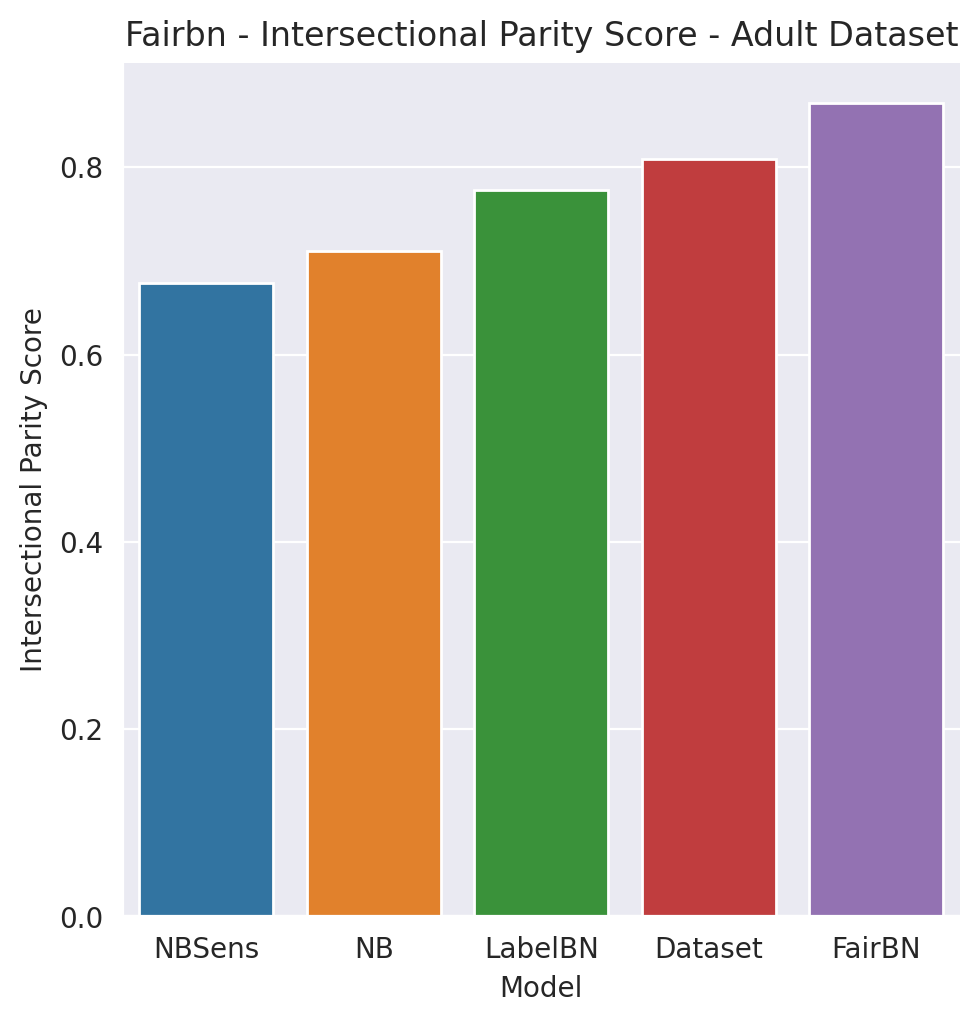
\includegraphics[width=0.49\linewidth]{figures/adult_fairbn_parity.png}
    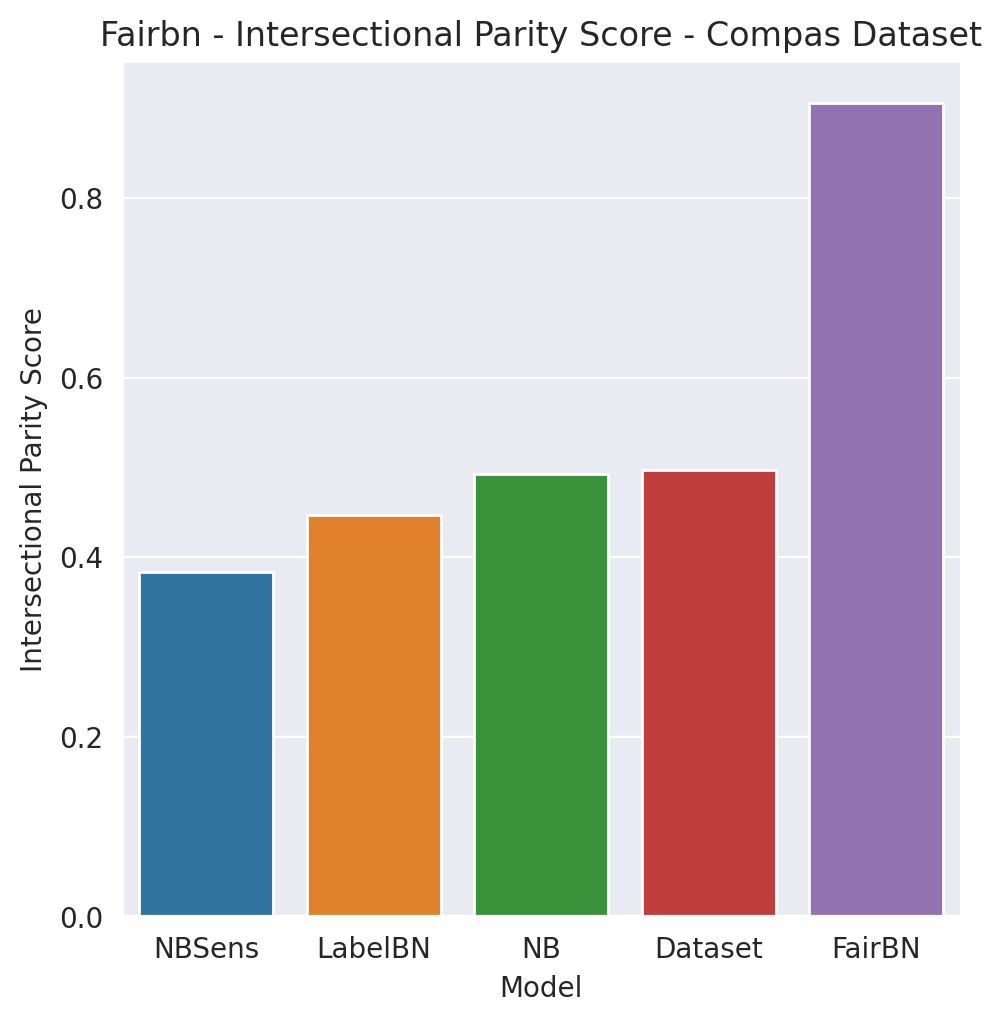
\includegraphics[width=0.49\linewidth]{figures/compas_fairbn_parity.png}
    \caption{Intersectional Parity Score for fair Bayesian network vs naïve bays.}
    \label{fig:exp1fairBNparity}
\end{figure}

\subsection{Fair Bayesian Network}

After training the fair Bayesian network classifier on the adult and Compas dataset, we get an intersectional parity score of $0.87$ and $0.91$ respectively. This is better than the inherent parity score in the dataset labels, which is $0.81$ and $0.51$ respectively. These results and how the different methods compare to one another is shown in figure~\ref{fig:exp1fairBNparity}.

In terms of accuracy and traditional performance of the model, we observe that there is a tradeoff between performance and fairness. This is best shown in the ROC curve shown in figure~\ref{fig:exp1fairBNROC}. There is a slight drop in the fair Bayesian network compared to the naïve Bayes method.

We also observe a quite significant performance difference between the adult dataset and the Compas dataset. Why this is is not explored further in this thesis, as we are interested in seeing differences in performance with respect to fairness.  
\begin{figure}
    \centering
    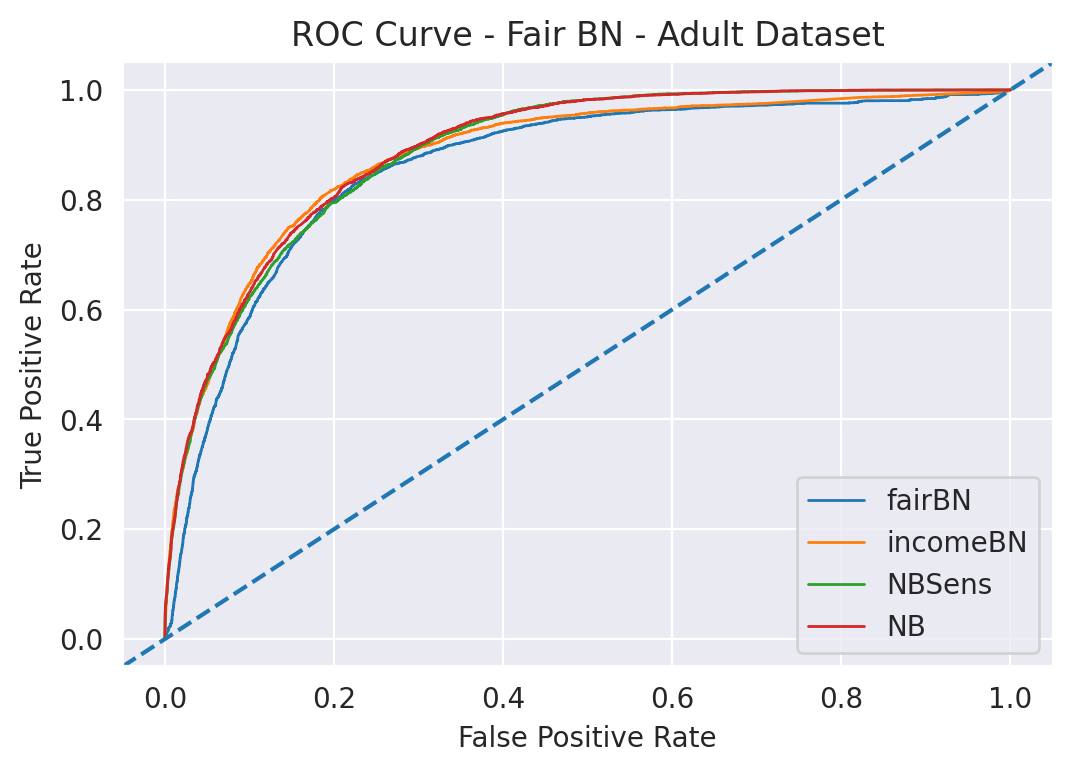
\includegraphics[width=0.49\linewidth]{figures/adult_fairbn_roc.png}
    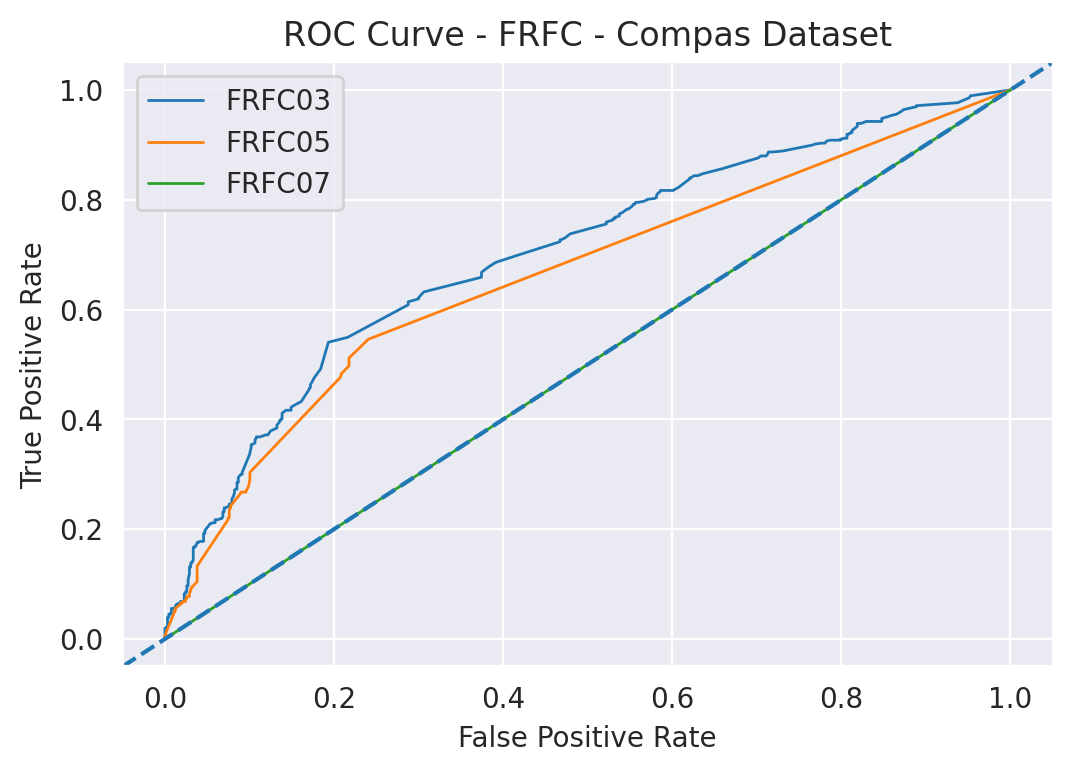
\includegraphics[width=0.49\linewidth]{figures/compas_frfc_roc.png}
    \caption{ROC curve for fair Bayesian network vs naïve Bayes.}
    \label{fig:exp1fairBNROC}
\end{figure}

\subsection{Fair Random Forest Classifier}

We ran the same experiments using their classifier on the adult dataset and Compas dataset. Rather interestingly, we do not observe any improvement in intersectional parity in the adult dataset for any of the methods, with the inherent intersectional parity for the dataset being $0.810$ and the best fair random forest classifier with $\Theta = 0.3$ having an intersectional parity of $0.78$, which is counterintuitive to the claimed meaning behind the hyperparameter $\Theta$ stated by the authors.

\begin{figure}
    \centering
    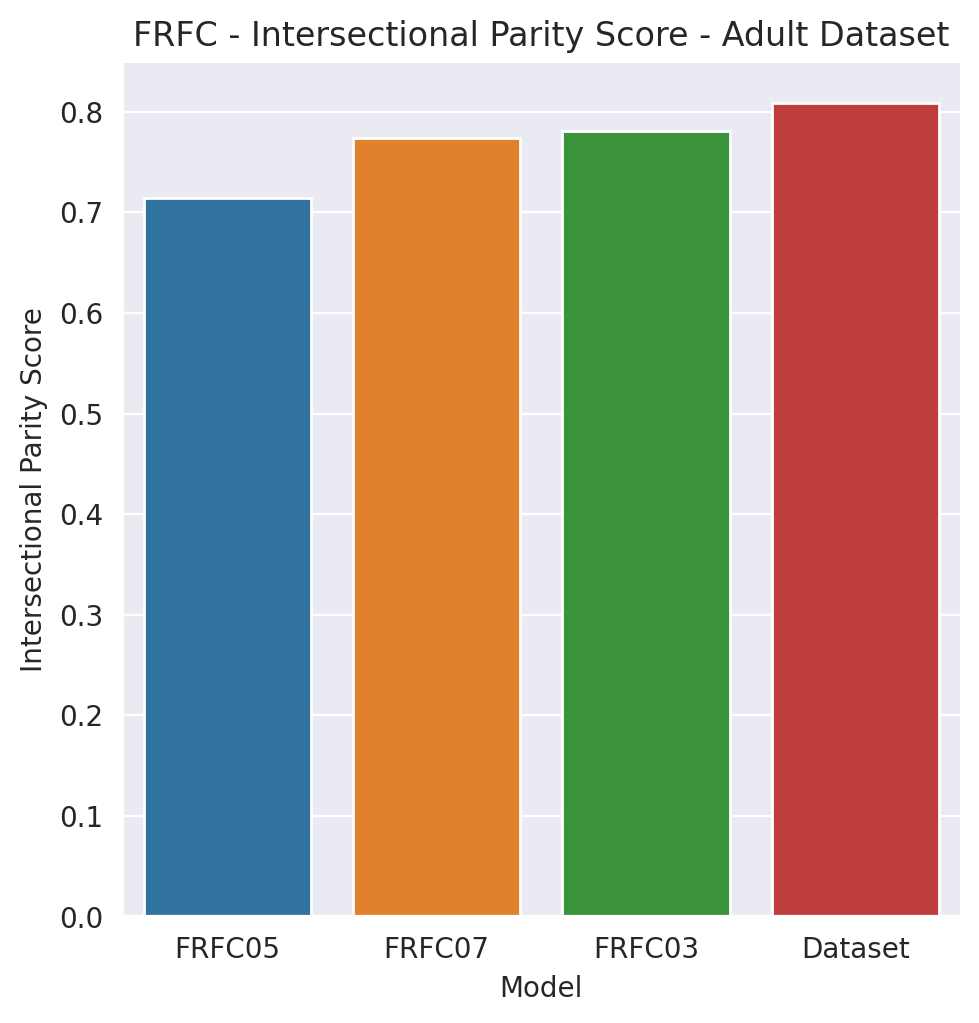
\includegraphics[width=0.49\linewidth]{figures/adult_frfc_parity.png}
    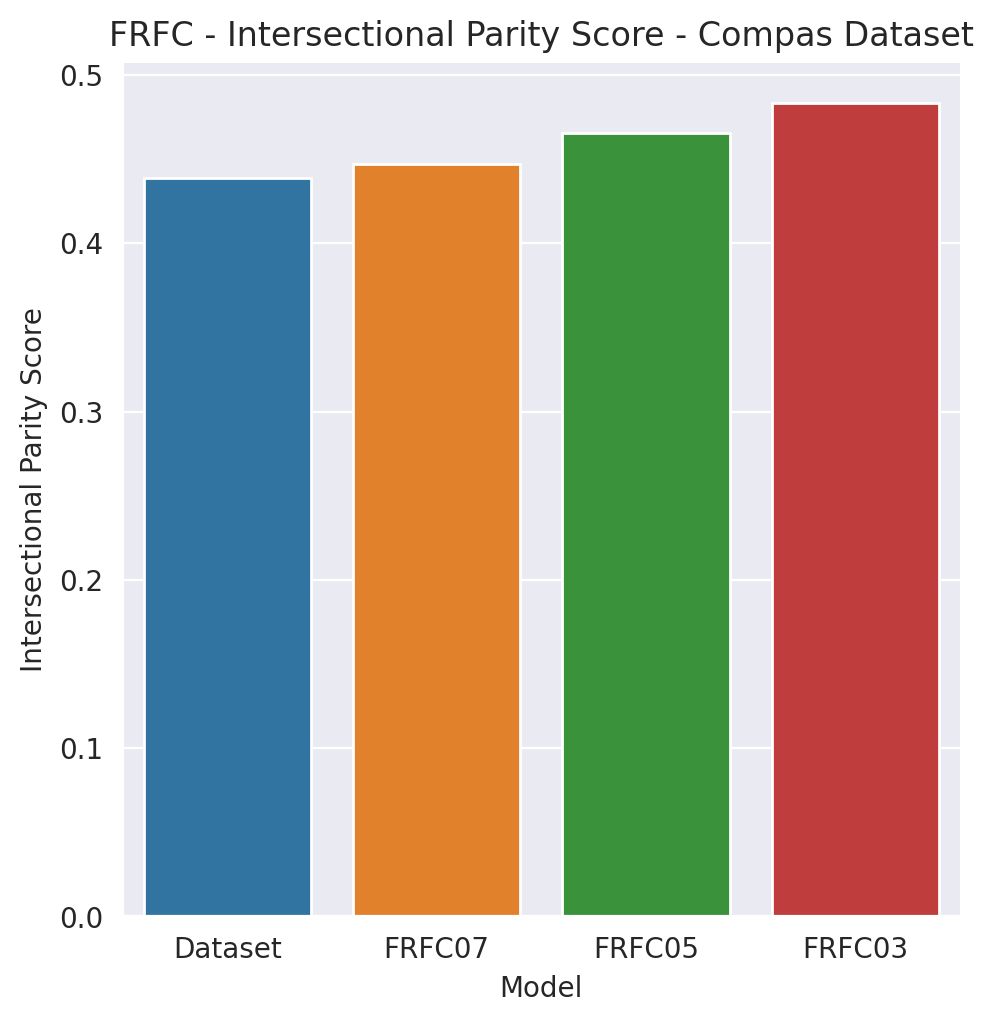
\includegraphics[width=0.49\linewidth]{figures/compas_frfc_parity.png}
    \caption{Parity score for fair random forest classifier.}
    \label{fig:exp1FRFCparity}
\end{figure}

For the Compas dataset, things are looking better with the models with $\Theta \in \{0.3, 0.7\}$ having higher intersectional parity scores than is inherent in the dataset labels. Still, the results given the stated meaning behind $\Theta$ is counterintuitive. The parity scores are shown in figure~\ref{fig:exp1FRFCparity}. The ROC curve for the different datasets is shown in figure~\ref{fig:exp1FRFCROC}

\begin{figure}
    \centering
    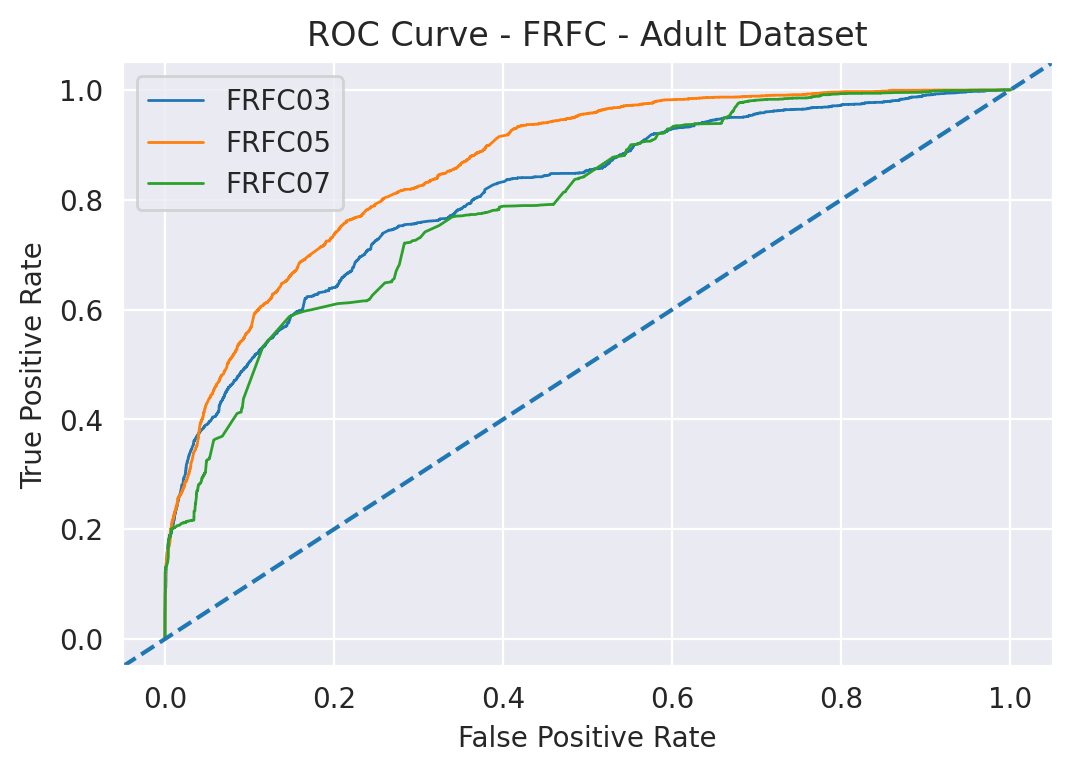
\includegraphics[width=0.49\linewidth]{figures/adult_frfc_roc.png}
    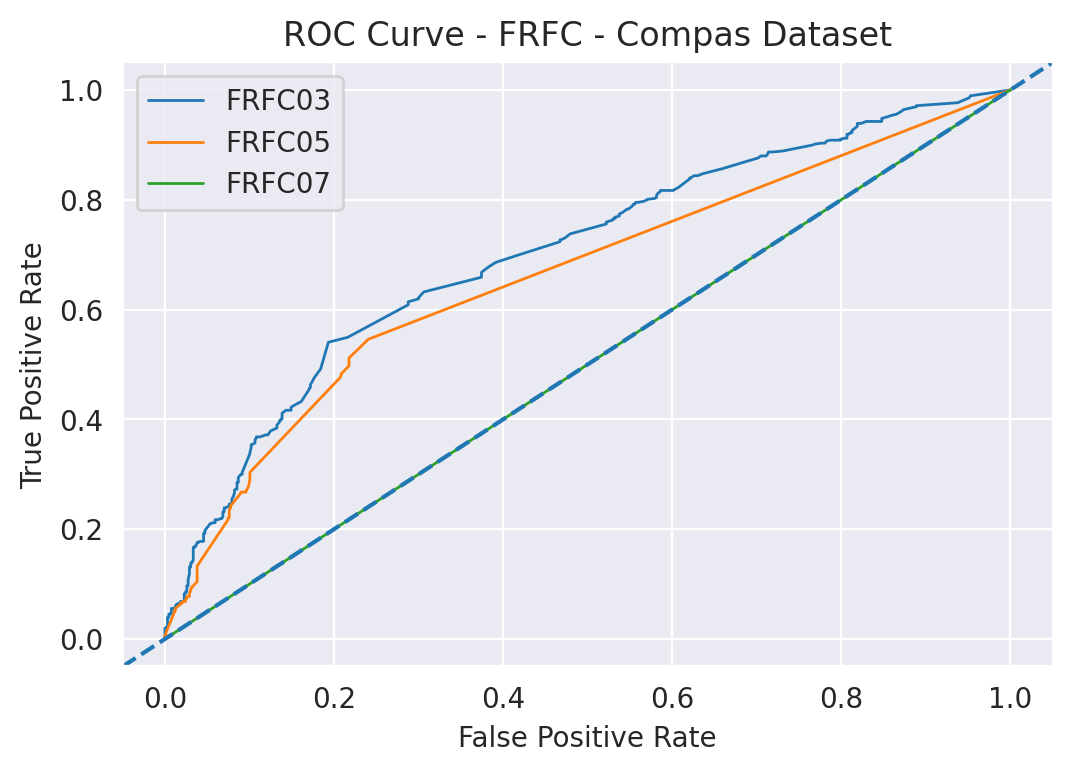
\includegraphics[width=0.49\linewidth]{figures/compas_frfc_roc.png}
    \caption{ROC curve for fair random forest classifier.}
    \label{fig:exp1FRFCROC}
\end{figure}

\section{Counterfactuals}

\subsection{naïve Bayes With Sensitive Attributes}

For the following datapoint:

\resizebox{\textwidth}{!}{
\begin{tabular}{lllllllllll}
\toprule
{} &           age & workclass &  education & marital-status &    occupation & relationship &   race &  gender &          capital-gain & hours-per-week \\
\midrule
46343 &  (31.6, 46.2] &   Private &  Assoc-voc &       Divorced &  Tech-support &    Unmarried &  Black &  Female &  (-4460.355, 16515.0] &   (20.6, 40.2] \\
\bottomrule
\end{tabular}
}

Got the following counterfactuals:

\resizebox{\textwidth}{!}{
\begin{tabular}{lllllllllllrrrr}
\toprule
{} &           age &  workclass &  education &     marital-status &    occupation &   relationship &                race &  gender &        capital-gain & hours-per-week &        O1 &   O2 &  O3 &   O4 \\
\midrule
155 &  (31.6, 46.2] &    Private &  Assoc-voc &  Married-AF-spouse &  Tech-support &      Unmarried &               Black &    Male &  (79128.0, 99999.0] &   (20.6, 40.2] &  0.000000 &  0.7 &   3 &  0.0 \\
162 &  (31.6, 46.2] &    Private &  Assoc-voc &           Divorced &  Adm-clerical &      Unmarried &               Black &    Male &  (79128.0, 99999.0] &   (20.6, 40.2] &  0.000000 &  0.7 &   3 &  0.0 \\
100 &  (31.6, 46.2] &    Private &  Assoc-voc &  Married-AF-spouse &  Adm-clerical &      Unmarried &               Black &    Male &  (58257.0, 79128.0] &   (20.6, 40.2] &  0.000000 &  0.6 &   4 &  0.0 \\
167 &  (31.6, 46.2] &    Private &  Assoc-voc &  Married-AF-spouse &  Adm-clerical &      Unmarried &               Black &    Male &  (79128.0, 99999.0] &   (20.6, 40.2] &  0.000000 &  0.6 &   4 &  0.0 \\
176 &  (31.6, 46.2] &    Private &  Assoc-voc &  Married-AF-spouse &  Adm-clerical &      Unmarried &               Black &    Male &  (58257.0, 79128.0] &   (20.6, 40.2] &  0.000000 &  0.6 &   4 &  0.0 \\
2   &  (60.8, 75.4] &  Local-gov &  Doctorate &           Divorced &             ? &  Not-in-family &  Amer-Indian-Eskimo &  Female &  (79128.0, 99999.0] &   (59.8, 79.4] &  0.000000 &  0.2 &   8 &  0.0 \\
177 &  (31.6, 46.2] &    Private &  Assoc-voc &  Married-AF-spouse &  Tech-support &      Unmarried &               Black &  Female &  (16515.0, 37386.0] &   (20.6, 40.2] &  0.419303 &  0.8 &   2 &  0.0 \\
\bottomrule
\end{tabular}
}


\instructions{
Page budget for Evaluation: 10-15 pages
%
\begin{itemize}
    \item Detail your evaluation methodology, present your results, and provide an analysis of them. Results can be quantitative and/or qualitative (from benchmark, user study, user satisfaction survey, etc.).
    \item It is strongly desired that you have empirical results, nevertheless, this may not be applicable to all types of theses.
\end{itemize}
}

\subsection{naïve Bayes Without Sensitive Attributes}

For the following datapoint:

\resizebox{\textwidth}{!}{
\begin{tabular}{lllllllllll}
\toprule
{} &             age & workclass & education & marital-status & occupation & relationship &   race &  gender &          capital-gain & hours-per-week \\
\midrule
23356 &  (16.927, 31.6] &         ? &   HS-grad &      Separated &          ? &    Unmarried &  Black &  Female &  (-4460.355, 16515.0] &   (20.6, 40.2] \\
\bottomrule
\end{tabular}
} 

We get the following counterfactuals:

\resizebox{\textwidth}{!}{
\begin{tabular}{lllllllllllrrrr}
\toprule
{} &             age &  workclass &  education &     marital-status & occupation &   relationship &                race &  gender &          capital-gain & hours-per-week &        O1 &   O2 &  O3 &   O4 \\
\midrule
128 &  (16.927, 31.6] &  State-gov &    HS-grad &          Separated &          ? &      Unmarried &               Black &    Male &    (79128.0, 99999.0] &   (20.6, 40.2] &  0.000000 &  0.7 &   3 &  0.0 \\
97  &    (31.6, 46.2] &          ? &    HS-grad &          Separated &          ? &  Not-in-family &               Black &    Male &    (79128.0, 99999.0] &   (20.6, 40.2] &  0.000000 &  0.6 &   4 &  0.0 \\
147 &  (16.927, 31.6] &  State-gov &  Doctorate &          Separated &          ? &      Unmarried &               Black &    Male &    (79128.0, 99999.0] &   (20.6, 40.2] &  0.000000 &  0.6 &   4 &  0.0 \\
136 &    (31.6, 46.2] &  State-gov &  Doctorate &  Married-AF-spouse &          ? &        Husband &  Amer-Indian-Eskimo &  Female &  (-4460.355, 16515.0] &   (20.6, 40.2] &  0.165877 &  0.4 &   6 &  0.1 \\
\bottomrule
\end{tabular}
}

\subsection{Fair Bayesian Network}

For the following counterfactual

\resizebox{\textwidth}{!}{
\begin{tabular}{lllllllllll}
\toprule
{} &             age & workclass & education & marital-status & occupation & relationship &   race &  gender &          capital-gain & hours-per-week \\
\midrule
23356 &  (16.927, 31.6] &         ? &   HS-grad &      Separated &          ? &    Unmarried &  Black &  Female &  (-4460.355, 16515.0] &   (20.6, 40.2] \\
\bottomrule
\end{tabular}
}

We get the following counterfactuals

\resizebox{\textwidth}{!}{
\begin{tabular}{lllllllllllrrrr}
\toprule
{} &             age &         workclass &   education & marital-status &       occupation &   relationship &                race &  gender &        capital-gain & hours-per-week &            O1 &   O2 &  O3 &   O4 \\
\midrule
111 &  (16.927, 31.6] &                 ? &        11th &      Separated &                ? &      Unmarried &               Black &  Female &  (79128.0, 99999.0] &   (79.4, 99.0] &  0.000000e+00 &  0.7 &   3 &  0.0 \\
114 &  (16.927, 31.6] &                 ? &     HS-grad &      Separated &                ? &      Unmarried &               White &  Female &  (79128.0, 99999.0] &   (79.4, 99.0] &  0.000000e+00 &  0.7 &   3 &  0.0 \\
162 &  (16.927, 31.6] &                 ? &        11th &      Separated &                ? &      Unmarried &               White &  Female &  (79128.0, 99999.0] &   (20.6, 40.2] &  0.000000e+00 &  0.7 &   3 &  0.1 \\
58  &  (16.927, 31.6] &      Never-worked &     HS-grad &      Separated &                ? &      Unmarried &  Asian-Pac-Islander &  Female &  (58257.0, 79128.0] &   (79.4, 99.0] &  0.000000e+00 &  0.6 &   4 &  0.0 \\
118 &  (16.927, 31.6] &                 ? &  Assoc-acdm &      Separated &                ? &      Unmarried &               Black &    Male &  (79128.0, 99999.0] &   (79.4, 99.0] &  0.000000e+00 &  0.6 &   4 &  0.0 \\
172 &  (16.927, 31.6] &      Never-worked &        11th &      Separated &                ? &      Unmarried &               White &  Female &  (58257.0, 79128.0] &   (20.6, 40.2] &  0.000000e+00 &  0.6 &   4 &  0.1 \\
\end{tabular}
}

\subsection{Fair Tree Classifier}


\section{Experimental Setup}
\label{sec:eval:expsetup}

\instructions{
\begin{itemize}
    \item Explain the methodology used for evaluating your contribution, and the metrics used for evaluation.
    \item If you use any dataset, explain it, detail its version, and mention briefly some main statistics about it, of interest for your problem (e.g., size, provenience, etc.), if appropriate.
    \item If you collect ground truth data, describe your annotation experiment. Explain what the annotators were asked to do (and show a screenshot or schema if available). Detail the number of annotators, their nature (experts, or crowdworkers), the criteria for deciding on each annotation instance (e.g., majority class, dynamic judgments, etc.), the criteria for ensuring quality (e.g., minimum accuracy, filters). If possible, report the inter-annotator agreement coefficient and mention how strong this value means that the agreement is.
\end{itemize}
}

\section{Experimental Results}
\label{sec:eval:results}


\instructions{
\begin{itemize}
    \item Present the results, using tables and (pretty) plots.
\end{itemize}
}

\section{Analysis}
\label{sec:eval:analysis}

\instructions{
\begin{itemize}
    \item Now that you presented the results, what do these results actually mean (esp. regarding the objectives you set out in the introduction)? 
    \item Can you identify success and failure cases? 
    \item What do the results say for individual parts you evaluate and overall in combination? 
    \item Make sure you formulate clear take-home messages.
\end{itemize}
}

\chapter{Conclusions}
\label{ch:conclusion}

\section{Summary of the thesis}

There is no question that fairness is important to incorporate in machine learning and decision-making systems if one wants to have the benefits of automation while at the same time achieve equality and sustainability for a better world. Machine learning model fairness and interpretability are vital for data scientists, researchers and developers to explain their models and understand the value and accuracy of their findings. Interpretability is also important to debug machine learning models and make informed decisions about how to improve them. While there exists many methods of achieving fairer systems, the field is still new and no state of the art exists. In this thesis, we have sought to investigate some current proposed methods for fair machine learning proposed in literature and try to shed some light on fairness in machine learning and what methods look promising or not. We have mainly focused on two approaches. The probabilistic Bayesian network approach and the fair tree classifier approach, which utilises two different methods for achieving fairness and also makes different assumptions. 

\subsection{Fair Bayesian Network}

The fair Bayesian network, proposed by \citet{Choi:2021:AIII}, which we have implemented in python using pgmpy in Forseti, makes the following assumptions

\begin{itemize}
    \item Training Data is biased
    \item The true fair class affiliation is a hidden attribute and must be inferred rather than measured.
    \item Demographic Parity is the definition of choice for fairness.
    \item Sensitive attributes are important in the decision-making process as they contain necessary information of context.
\end{itemize}

\subsection{Fair Tree Classifiers}

While the fair tree classifier makes the following assumptions

\begin{itemize}
    \item Training data is used as the true state of nature.
    \item Strong Demographic Parity is the definition of choice for fairness.
    \item Sensitive attributes should not be used during inference and used to evaluate splits during the training phase. Penalising the split if the sensitive attribute depends on the outcome.
\end{itemize}

\subsection{Approach}

We have trained these models extensively on the Adult dataset and COMPAS dataset which are established datasets in fairness research. We have proposed new performance metrics that incorporate fairness and evaluated models in terms of this. To validate these new metrics, we have proposed new algorithms for generating datasets where we are in control of the bias in the data to further evaluate these metrics.

In addition to training models and evaluating them in terms is new proposed fairness measures, we have tried to explicitly explain and understand the behaviour of the models to validate that models satisfying fairness measures actually truly achieves fair behaviour. In addition we have implemented an genetic algorithm approach to generate counterfactual data points that highlight what attribute changes flip the outcome of an individual. Which gives a quite intuitive overview of the inner workings of the models.

\section{Findings}

We have observed quite different behaviour from the two approaches investigated, while both claim to achieve fairness in their predictions, we have only been able to replicate these results with the approach proposed by \citet{Choi:2021:AIII}. In the approach proposed by \citet{Antonio:2021:arXiv} we have not been able to replicate the results presented in their paper.

From our work, we have shown that the fair Bayesian network is able to achieve fairer predictions while not suffering too much from the fairness-accuracy tradeoff. There is still a tradeoff, and the model does not achieve the same performance in terms of traditional performance measures as the naïve Bayes model. This is reasonable and expected from the model given that the model assumes that the dataset labels are biased and incorrect and only used to infer the true state of nature. 

By employing machine learning interpretability methods, we have also shown that the fair Bayesian network achieves its fairness through affirmative actions. This is done by increasing the predictive probability of a fairer outcome, while giving neglected groups a higher chance of a positive outcome than expected from their representation in the training data.

From the same approach when looking at the fair tree classifier, we see a very high variation in the performance of the model in terms of fairness while traditional performance metrics are not high enough to confidently determine that the distribution of predictions better than predicting at random. Suggesting that the model achieves its fairness performance by predicting randomly. 

This shows that Demographic Parity as an performance metric might at first seem intuitive and well defined, but as with any optimisation problem, it is very hard defining good objective function that makes a model achieve what you really want. The easiest way to achieve demographic parity is to reject any model and just sample predictions at random, giving predictions that are independent of the sensitive attributes but in no sense an informed prediction.

\section{Research Questions}

\subsection{RQ1: What probabilistic graphical model is most appropriate to model the discrimination process?}

We believe that we have demonstrated the power of graphical models through their intuitive design and graphical representation of their conditional probabilities and dependencies between variables to make them fit for use for fair machine learning. Inferring latent class affiliations from datasets that are assumed to be biased is probably a quite reasonable assumption, and a necessary one to achieve fairness. Probabilistic Graphical Models may have a future as the model of choice when it comes to fair machine learning.

\subsection{RQ2: Are the proposed models explainable?}

The proposed models are not fully interpretable. The fair random forest is not interpretable and given that the model does not use the sensitive attributes in it's predictions, it is hard to infer the inner workings and decision making of the model through model-agnostic interpretability methods. The fair Bayesian network is to a more extent interpretable, dependent on the complexity of the Bayesian network. In the case that the model is an naïve Bayes classifier it is quite intuitive for a human to understand how each attribute contributes to the outcome. As the complexity of the Bayesian network increases, this becomes more difficult. 

\subsection{RQ3: Are probabilistic machine learning models cost-effecitive?}

While we have not discussed this in detail, the biggest challenge to the probabilistic graphical model approach is that inference is a NP-Hard problem and requires quite a lot of computing resources. The inference is thus very slow. For some real-world cases out there this could make such models infeasible. This is the biggest drawback to these models. 

\section{Future Directions}
\label{sec:conclusions:future}

For future work, exploring new graphical models should be encouraged. The number of possible graphical models out there is vast and given the performance these can achieve this could lead to some interesting new models. Additionally, while inference in the graphical models used here is NP-Hard, sum-product networks do not suffer with this problem having very fast inference and probabilistic calculations. Implementing fair graphical models as sum-product networks and developing libraries for this could improve the ease of implementation as well as increase the cost-effectiveness of such models.

From our results we also see that demographic parity alone as a definition of fairness can lead to models having undesired behaviour. Investigating further definitions of fairness for machine learning should be in focus. If one would find a performance metric that truly achieve fairness, a lot of models could very quickly be adapted to incorporate fairness. 

We have also shown that until a state of the art fair performance metric exist, machine learning interpretability will be necessary to evaluate models in terms of fairness and to avoid accidentally deploying bad models even though they achieve good performances. Developing a framework and methods for incorporating fair machine learning methods together with machine learning interpretability should be explored further.

%% ----------------------------------------------------------------
% Now begin the Appendices, including them as separate files

\addtocontents{toc}{\vspace{2em}} % Add a gap in the Contents, for aesthetics

\appendix % Cue to tell LaTeX that the following 'chapters' are Appendices
\chapter{Experimental results, figures and poster}

\section{Experiment 1 Results}
\label{app:experiment1}

\begin{landscape}
\begin{table}[H]
\centering
\begin{tabular}{|l|l|l|l|l|l|l|l|l|}
\hline
\textbf{Accuracy} & \textbf{BA} & \textbf{F1 Score} & \textbf{Specificity} & \textbf{PS Race} & \textbf{PS gender} & \textbf{Int PS} & \textbf{Model} & \textbf{Dataset} \\ \hline
0.42000 & 0.61000 & 0.45000 & 0.24000 & 0.88000 & 0.80000 & 0.77000 & FRFC07      & Adult  \\ \hline
0.54000 & 0.65000 & 0.47000 & 0.44000 & 0.88000 & 0.79000 & 0.78000 & FRFC03      & Adult  \\ \hline
0.66000 & 0.75000 & 0.57000 & 0.58000 & 0.86000 & 0.67000 & 0.71000 & FRFC05      & Adult  \\ \hline
0.81000 & 0.80000 & 0.67000 & 0.83000 & 0.82000 & 0.66000 & 0.71000 & NBSens      & Adult  \\ \hline
0.81000 & 0.80000 & 0.67000 & 0.83000 & 0.82000 & 0.66000 & 0.71000 & NBSens      & Adult  \\ \hline
0.82000 & 0.76000 & 0.63000 & 0.89000 & 0.88000 & 0.94000 & 0.87000 & FairBN      & Adult  \\ \hline
0.83000 & 0.72000 & 0.59000 & 0.94000 & 0.85000 & 0.75000 & 0.78000 & IncomeBN    & Adult  \\ \hline
1.00000 & 1.00000 & 1.00000 & 1.00000 & 0.85000 & 0.80000 & 0.81000 & Dataset     & Adult  \\ \hline
0.60000 & 0.56000 & 0.28000 & 0.96000 & 0.94000 & 0.90000 & 0.91000 & FairBN      & Compas \\ \hline
0.60000 & 0.57000 & 0.28000 & 0.96000 & 0.95000 & 0.66000 & 0.45000 & LabelBN     & Compas \\ \hline
0.64000 & 0.62000 & 0.52000 & 0.81000 & 0.70000 & 0.56000 & 0.38000 & NBSensitive & Compas \\ \hline
0.64000 & 0.64000 & 0.61000 & 0.64000 & 0.91000 & 0.54000 & 0.49000 & NB          & Compas \\ \hline
1.00000 & 1.00000 & 1.00000 & 1.00000 & 0.94000 & 0.54000 & 0.50000 & Dataset     & Compas \\ \hline
0.53000 & 0.56000 & 0.64000 & 0.20000 & 0.99000 & 0.82000 & 0.82000 & FRFC03      & Compas \\ \hline
0.61000 & 0.59000 & 0.39000 & 0.91000 & 0.90000 & 0.66000 & 0.45000 & FRFC05      & Compas \\ \hline
0.46000 & 0.50000 & 0.63000 & 0.00000 & 1.00000 & 1.00000 & 1.00000 & FRFC07      & Compas \\ \hline
\end{tabular}
\end{table}
\end{landscape}

\section{Poster}
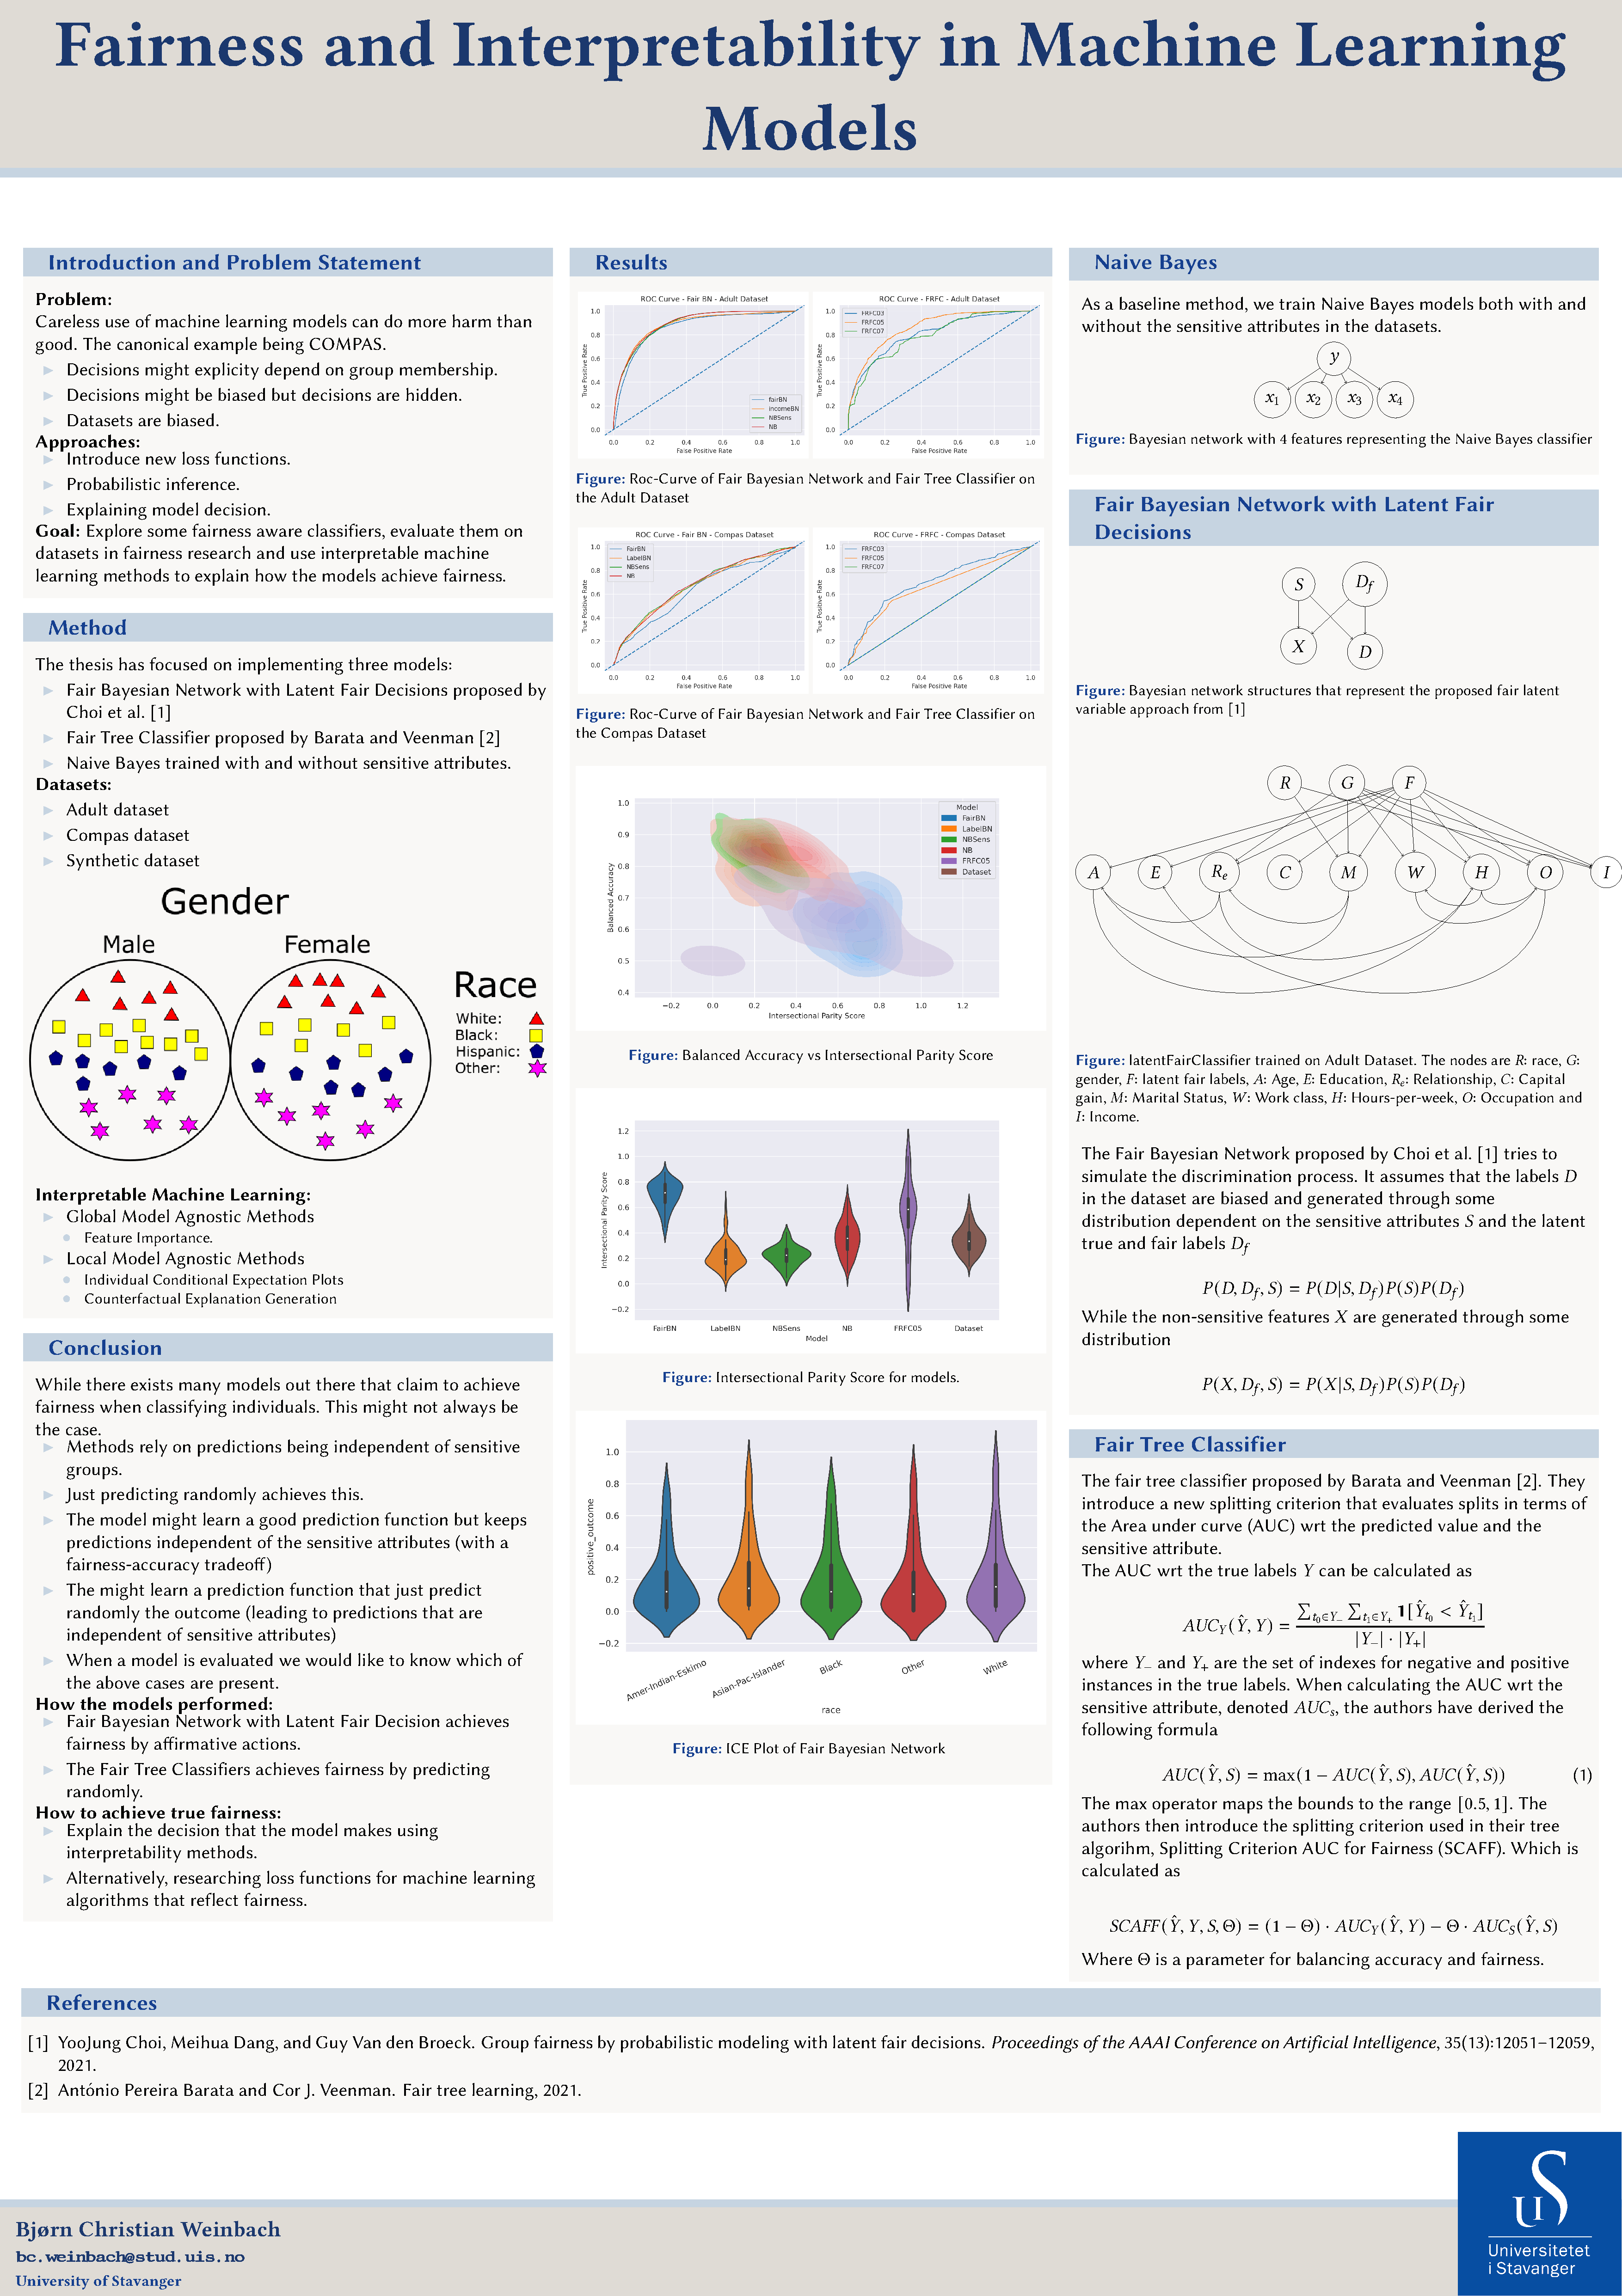
\includepdf[width=\linewidth]{MDAT_Thesis_Poster_Weinbach.pdf}
\chapter{Instructions to Compile and Run System}
\label{apx:instructions}

\section{Installation Instructions}

The code used in this thesis is organised in Jupyter notebooks and it is programmed using python. A range of libraries is used and these are managed using Anaconda\footnote{https://www.anaconda.com/}. To make it as easy as possible to recreate the environment, we suggest that Anaconda is installed so the environment can be recreated easily. Installing anaconda is explained in detail in the documentation\footnote{https://docs.anaconda.com/anaconda/install/}.

\subsection{The Python Environment}

It is not mandatory to install anaconda to run the code. The libraries that are necessary are as follows:

\begin{itemize}
    \item Python
    \item Pytest
    \item Flake8 (Used for linting)
    \item Black (Used for linting and formatting)
    \item jupyter
    \item ipykernel
    \item pandas
    \item seaborn
    \item pip
    \item installed using pip: pgmpy
\end{itemize}

As long as these libraries are installed the code should work. 

\subsection{Setting up the environment using Anaconda}

After installing Anaconda. The environment is set up as follows. 

\begin{enumerate}
    \item Navigate to the root folder of the code repository. There you should find a file named \emph{environment.yml}.
    \item Run the command: \emph{conda env create -f environment.yml}
    \item When the previous command is complete. Run \emph{conda acitvate forseti} to activate the environment.
\end{enumerate}

Now the environment is active and running and ready to execute the code.

\subsection{Notebooks}

We will go through each of the notebooks and their purpose so you know which notebook to use if you want to reproduce results.

\begin{itemize}
    \item Bayesian-net-adult: Notebook used to train the fair bayesian network and naive bayes classifiers as well as saving predictions on the adult dataset.
    \item Counterfactuals: Runs the \emph{generateCounterfactuals} method on the trained naive bayes and fair bayesian networks and export the results to latex
    \item data\_exploration: Early notebook for exploring the adult dataset. Calculate correlation for dummy variables and plot the results.
    \item experiment2-visualisation: Generates a synthetic dataset, traind models on the synthetic dataset and visualises their scores.
    \item fairtree: Training the fair tree classifier on the adult dataset and COMPAS dataset and store its predictions.
    \item Interpretability: Training of simple interpretable models, and calculating feature importance for implemented models.
    \item Local-agnostic: Visualise ICE plots for implemented models.
    \item Model-evaluation: Calculate fairness scores for adult dataset on the implemented models.
\end{itemize} 

\addtocontents{toc}{\vspace{2em}}  % Add a gap in the Contents, for aesthetics
\backmatter

%% ----------------------------------------------------------------
\label{Bibliography}
\lhead{\emph{Bibliography}}  % Change the left side page header to "Bibliography"
\bibliographystyle{unsrtnat}  % Use the "unsrtnat" BibTeX style for formatting the Bibliography
\bibliography{Bibliography}  % The references (bibliography) information are stored in the file named "Bibliography.bib"

\end{document}
